\documentclass[12pt]{report}
\usepackage{xcolor}
\usepackage[utf8]{inputenc}
\usepackage{natbib}
\usepackage[left=1.25in,right=1.0in,top=1.0in,bottom=1.0in]{geometry}
\usepackage{float}
\linespread{1.3}
\usepackage{graphicx}
\usepackage{rotating}
\usepackage{amsmath,amssymb}
\usepackage{titlesec}
\usepackage{tabularx}
\usepackage{booktabs}
\usepackage{enumitem}
\usepackage[hidelinks]{hyperref}
\usepackage{url}
\usepackage{tikz}
\usetikzlibrary{shapes.geometric, arrows, positioning, fit, calc}

%--- Chapter/section formatting (match department template) ---
\titlespacing*{\chapter}{-15pt}{10pt}{15pt}
\titlespacing*{\section}{0pt}{0pt}{5pt}
\titlespacing*{\subsection}{0pt}{5pt}{5pt}
\titleformat{\chapter}[hang]
{\normalfont\huge\bfseries}{\chaptertitlename\ \thechapter.}{1em}{}
\renewcommand{\chaptername}{}

\graphicspath{{Images/}}

\begin{document}

% ===========================
% Custom Title Page
% ===========================
\begin{titlepage}
\begin{center}
    
\includegraphics[scale=.3]{logotu.jpg}\\[0.5cm]
    {\large \textbf{TRIBHUVAN UNIVERSITY}}\\
    {\large \textbf{INSTITUTE OF ENGINEERING}}\\
    {\large \textbf{PULCHOWK CAMPUS}}\\[0.8cm]
    {\large A Project Report On}\\[0.3cm]
    {\Large \textbf{Project/Thesis Management System (TPMS)}}\\[0.8cm]
    {\large \textbf{Submitted By:}}\\[0.2cm]
    {\large Prabesh BC (PUL080BCT054)}\\
    {\large Shreeyut Thapa (PUL080BCT080)}\\
    {\large Subesh Yadav (PUL080BCT084)}\\[0.8cm]
    {\large \textbf{Submitted To:}}\\[0.2cm]
    {\large Department of Electronics \& Computer Engineering}\\[0.3cm]
    {\large In Partial Fulfillment of the Requirements for the Degree of}\\
    {\large Bachelor of Engineering in Computer Engineering}\\[0.8cm]
    {\large \textbf{DEPARTMENT OF ELECTRONICS \& COMPUTER ENGINEERING}}\\
    {\large Lalitpur, Nepal}\\[0.3cm]
    {\large August, 2026}
\end{center}
\end{titlepage}
\pagenumbering{roman}
\setcounter{page}{2}

%===========================
% Page of Approval
%===========================
\chapter*{Page of Approval}
\addcontentsline{toc}{chapter}{\numberline{}Page of Approval}
\vspace{1.5cm}
\begin{center}
\uppercase{
Tribhuvan University\\
Institute of Engineering\\
Pulchowk Campus\\
Department of Electronics and Computer Engineering
}
\end{center}
\vspace{.5cm}
The undersigned certifies that they have read and recommended to the Institute of Engineering for acceptance of a project report entitled \textbf{``Project/Thesis Management System (TPMS)''} submitted by \textbf{Prabesh BC}, \textbf{Shreeyut Thapa}, and \textbf{Subesh Yadav} in partial fulfillment of the requirements for the Bachelor's degree in Electronics \& Computer Engineering.\\

\vspace{1cm}
\begin{minipage}{.5\textwidth}
    \raggedright
    .............................\\
    Supervisor\\
    \textbf{Supervisor Full Name}\\
    Designation, Department of Electronics and Computer Engineering,\\
    Pulchowk Campus, IOE, TU.\\
\end{minipage}%
\begin{minipage}{0.5\textwidth}
    \raggedleft
    .............................\\
    External Examiner\\
    \textbf{Examiner Full Name}\\
    Assistant Professor\\
    Department of Electronics and Computer Engineering,\\
    Pulchowk Campus, IOE, TU.\\
\end{minipage}\\
\newline
\newline
\newline
\centerline{Date of approval:}

%===========================
% Copyright
%===========================
\chapter*{Copyright}
\addcontentsline{toc}{chapter}{\numberline{}Copyright}
The author has agreed that the Library, Department of Electronics and Computer Engineering, Pulchowk Campus, and Institute of Engineering may make this report freely available for inspection. Moreover, the author has agreed that permission for extensive copying of this project report for scholarly purposes may be granted by the supervisors who supervised the work recorded herein or, in their absence, by the Head of the Department wherein the project report was done. It is understood that recognition will be given to the author of this report and the Department of Electronics and Computer Engineering, Pulchowk Campus, Institute of Engineering for any use of the material of this project report. Copying, publication, or other use of this report for financial gain without the approval of the Department of Electronics and Computer Engineering, Pulchowk Campus, Institute of Engineering, and the author's written permission is prohibited.\\
Request for permission to copy or to make any other use of the material in this report in whole or in part should be addressed to:\\
\newline
\newline
\newline
Head\\
Department of Electronics and Computer Engineering\\
Pulchowk Campus, Institute of Engineering, TU\\
Lalitpur, Nepal.

%===========================
% Acknowledgements
%===========================
\chapter*{Acknowledgements}
\addcontentsline{toc}{chapter}{\numberline{}Acknowledgements}
We would like to express our profound gratitude to our project supervisor, \textbf{[Supervisor Full Name]}, Department of Electronics and Computer Engineering, Pulchowk Campus, for their continuous guidance, constructive feedback, and unwavering support throughout the entire development lifecycle of this project. Their technical insights and pedagogical direction were instrumental in shaping the architecture and quality of the Thesis and Project Management System.

We are deeply grateful to the \textbf{Department of Electronics and Computer Engineering, Pulchowk Campus, Institute of Engineering, Tribhuvan University}, for providing the academic framework, laboratory infrastructure, and institutional context that made this project possible.

We extend our sincere thanks to all faculty members and staff of DOECE who participated in User Acceptance Testing sessions and provided candid operational feedback that significantly improved the system's usability and functional coverage.

We are also thankful to our fellow classmates and student peers who volunteered their time to validate the student-facing group formation and document submission workflows.

Finally, we wish to express our deepest appreciation to our families for their constant moral support and encouragement throughout the duration of this program.

%===========================
% Abstract
%===========================
\chapter*{Abstract}
\addcontentsline{toc}{chapter}{\numberline{}Abstract}
The Project/Thesis Management System (TPMS) is a production-grade, role-aware web platform developed for the Department of Electronics and Computer Engineering (DOECE), Pulchowk Campus, Institute of Engineering, Tribhuvan University. The system digitalizes and automates the complete administrative and evaluative lifecycle of Bachelor Minor and Major projects and Master research theses across six academic programs (BCT, BEI, MSCSK, MSICE, MSDSA, MSNCS), replacing existing manual, paper-based workflows.

The platform enforces a five-role hierarchy (Maintainer, Coordinator, Supervisor, Student, External Examiner) governed by Role-Based Access Control (RBAC) and strict program-scoped degree isolation. A Global Engagement Guard prevents students from enrolling in multiple active project groups simultaneously, while an automated Conflict-of-Interest Filter ensures that assigned supervisors cannot serve as defense evaluators for their own projects. The system implements the DOECE evaluation schemes (Minor: 50 marks; Major: 100 marks; Master Thesis: 300 marks) through a dynamic rubric engine.

A server-side Puppeteer headless Chrome pipeline generates official A4 PDF grade sheets with automated number-to-words mark conversion. A SheetJS-powered Excel bulk import pipeline with pre-commit anomaly detection enables large-scale student onboarding. A program-scoped audit trail provides tamper-evident event logging for institutional accountability.

The system is implemented with React 18 and Vite 5 on the frontend, Node.js and Express.js on the backend, and PostgreSQL 16 managed via Prisma 5 ORM. Evaluation through unit testing (36 tests, 100\% pass rate), integration testing, security testing, and User Acceptance Testing (average satisfaction 4.47/5.0) confirmed functional completeness and operational readiness. All API endpoints responded within 300 ms under test load, and PDF generation completed within 2 seconds.\\
\newline
Keywords: \textit{Academic Project Management, Role-Based Access Control, Evaluation Rubric Engine, PDF Grade Sheet Generation, Conflict-of-Interest Prevention, Node.js, React, PostgreSQL, Prisma ORM}

%===========================
% Tables of Contents / Figures / Tables
%===========================
\tableofcontents
\addcontentsline{toc}{chapter}{\numberline{}Contents}
\listoffigures
\addcontentsline{toc}{chapter}{\numberline{}List of Figures}
\listoftables
\addcontentsline{toc}{chapter}{\numberline{}List of Tables}

%===========================
% List of Abbreviations
%===========================
\chapter*{List of Abbreviations}
\addcontentsline{toc}{chapter}{\numberline{}List of Abbreviations}
\begin{tabular}{l l}
\textbf{API} & Application Programming Interface \\
\textbf{BCT} & Bachelor of Computer Engineering \\
\textbf{BEI} & Bachelor of Electronics, Communication and Information Engineering \\
\textbf{CRUD} & Create, Read, Update, Delete \\
\textbf{CSS} & Cascading Style Sheets \\
\textbf{COI} & Conflict of Interest \\
\textbf{DOECE} & Department of Electronics and Computer Engineering \\
\textbf{DFD} & Data Flow Diagram \\
\textbf{HTTP} & Hypertext Transfer Protocol \\
\textbf{IOE} & Institute of Engineering \\
\textbf{JWT} & JSON Web Token \\
\textbf{MSDSA} & Master of Science in Data Science and Analytics \\
\textbf{MSICE} & Master of Science in Information and Communication Engineering \\
\textbf{MSCSK} & Master of Science in Computer Systems and Knowledge Engineering \\
\textbf{MSNCS} & Master of Science in Network and Cyber Security \\
\textbf{MVC} & Model-View-Controller \\
\textbf{ORM} & Object-Relational Mapping \\
\textbf{PDF} & Portable Document Format \\
\textbf{RBAC} & Role-Based Access Control \\
\textbf{REST} & Representational State Transfer \\
\textbf{SPA} & Single-Page Application \\
\textbf{SQL} & Structured Query Language \\
\textbf{TPMS} & Thesis and Project Management System \\
\textbf{TU} & Tribhuvan University \\
\textbf{UAT} & User Acceptance Testing \\
\textbf{UI} & User Interface \\
\textbf{UML} & Unified Modeling Language \\
\textbf{UX} & User Experience \\
\textbf{VPS} & Virtual Private Server \\
\end{tabular}

%===========================
% Chapters (Arabic numbering starts at Ch1)
%===========================
\chapter{Introduction}
\pagenumbering{arabic}

\section{Background}
Academic project and thesis coursework represent pivotal milestones in engineering curricula at Tribhuvan University (TU), Institute of Engineering (IOE), Pulchowk Campus. Under the Department of Electronics and Computer Engineering (DOECE), undergraduate students enrolled in Bachelor of Computer Engineering (BCT) and Bachelor of Electronics, Communication and Information Engineering (BEI) undertake compulsory Minor and Major projects during their third and fourth academic years. Concurrently, postgraduate scholars across specialized Master of Science programs---including Computer Systems and Knowledge Engineering (MSCSK), Information and Communication Engineering (MSICE), Data Science and Analytics (MSDSA), and Network and Cyber Security (MSNCS)---execute multi-semester research theses.

Historically, the administrative, supervisory, and evaluative management of these academic initiatives has relied almost exclusively on manual, fragmented, and paper-intensive procedures. Departmental coordinators have had to physically gather proposal drafts, manually record group rosters into ad-hoc spreadsheets, collect printed mid-term and final reports, and distribute handwritten evaluation marking rubrics during formal defense sessions. As student enrollment and specialized postgraduate programs have grown, this legacy operational model has created significant administrative strain, operational bottlenecks, scheduling conflicts, and data inconsistencies.

Modern higher education institutions increasingly leverage specialized academic information systems to govern collaborative workflows, ensure institutional accountability, and maintain transparent audit trails~\citep{pressman2015software, ko2021systematic}. The \textbf{Thesis and Project Management System (TPMS)} is developed as an enterprise-grade, web-based platform engineered specifically to digitalize, govern, and streamline the complete lifecycle of Bachelor projects and Master theses at DOECE, Pulchowk Campus. By incorporating strict degree isolation, automated conflict-of-interest prevention, dynamic evaluation rubric computation, server-side grade sheet rendering, and program-scoped audit logging, TPMS replaces disparate manual processes with a unified digital ecosystem.

\section{Problem Statement}
The prevailing manual and spreadsheet-dependent methodology employed for project and thesis governance at DOECE presents multiple systemic inefficiencies and structural challenges:

\begin{enumerate}[label=\textbf{P\arabic*.}]
    \item \textbf{Decentralized and Fragmented Record-Keeping:} Project records, student team rosters, supervisor allocations, and proposal drafts reside across disconnected physical binders, local spreadsheets, and unstructured email exchanges. This fragmentation prevents coordinators and department leadership from gaining real-time operational visibility into project progress and milestone completion.
    
    \item \textbf{Lack of Systemic Multi-Project Engagement Controls:} In manual systems, cross-checking whether a student has registered in multiple project groups or enrolled simultaneously in conflicting teams requires exhaustive manual auditing across spreadsheets. The absence of automated validation allows accidental double-registration and invalid group compositions.
    
    \item \textbf{Vulnerability to Supervisory Conflicts of Interest:} During mid-term and final defense sessions, faculty members who supervise a project must not be designated as external or internal evaluating examiners for that identical project. Manually cross-referencing examiner schedules against supervisor allocations across hundreds of students is error-prone, creating potential ethical and academic evaluation conflicts.
    
    \item \textbf{Manual Mark Tabulation and Inconsistent Evaluation Schemes:} Bachelor Minor (50 marks), Bachelor Major (100 marks), and Master Theses (300 marks) adhere to distinct evaluation components distributed across supervisors, defense committees, internal examiners, and external evaluators. Manually compiling scores, verifying sub-criteria limits, and converting marks into official text representations is labor-intensive and susceptible to human calculation errors.
    
    \item \textbf{Cumbersome Official Documentation and Grade Sheet Compilation:} Departmental guidelines require official, standardized A4 evaluation sheets bearing institutional letterheads, committee signature panels, and student rosters for submission to the TU Examination Control Division. Manually typesetting these sheets for dozens of groups introduces formatting disparities and substantial delays.
    
    \item \textbf{Absence of Immutable Audit Logging and Security Controls:} Manual document handovers and email submissions lack tamper-proof timestamping and role-based access restrictions, making it difficult to verify submission deadlines, document version histories, and faculty actions.
\end{enumerate}

\section{Objectives}

\subsection{Main Objective}
The primary objective of this project is to design, develop, and evaluate a secure, role-aware, and production-grade \textbf{Project/Thesis Management System (TPMS)} that automates and digitalizes the end-to-end academic project lifecycle for undergraduate and postgraduate programs under the Department of Electronics and Computer Engineering, Pulchowk Campus.

\subsection{Specific Objectives}
To achieve the primary objective, the following specific objectives are established:
\begin{enumerate}[label=\arabic*.]
    \item To architect a multi-role web platform supporting five distinct stakeholder roles (\textit{Maintainer}, \textit{Coordinator}, \textit{Supervisor}, \textit{Student}, and \textit{External Examiner}) governed by Role-Based Access Control (RBAC) and program-level degree isolation.
    \item To implement a robust team formation and proposal registration subsystem equipped with an automated \textit{Engagement Guard} to prevent multi-project enrollments and enforce team size limits (1--4 students for Bachelor projects; 1 student for Master theses).
    \item To develop a centralized Coordinator Response Matrix with live fuzzy supervisor matching, deduplicated group views, and inline lifecycle finalization.
    \item To build an automated \textit{Conflict-of-Interest Filter} that dynamically excludes assigned project supervisors from acting as internal or external defense examiners on their supervised projects.
    \item To engineer a dynamic, stage-wise rubric evaluation engine tailored to the DOECE grading schemes for Minor Projects (50 marks), Major Projects (100 marks), and Master Theses (300 marks).
    \item To integrate a server-side headless browser rendering pipeline for instant, pixel-perfect generation of official TU Pulchowk Campus evaluation sheets and consolidated grade reports with automated number-to-words conversion.
    \item To construct an Excel-based bulk data ingestion pipeline with pre-validation anomaly detection alongside a program-scoped audit logging mechanism.
\end{enumerate}

\section{Scope and Limitations}

\subsection{Scope of the Project}
The operational scope of the TPMS encompasses the academic and administrative activities of DOECE, Pulchowk Campus:
\begin{itemize}
    \item \textbf{Academic Programs Covered:} Bachelor of Computer Engineering (BCT), Bachelor of Electronics, Communication and Information Engineering (BEI), MS in Computer Systems and Knowledge Engineering (MSCSK), MS in Information and Communication Engineering (MSICE), MS in Data Science and Analytics (MSDSA), and MS in Network and Cyber Security (MSNCS).
    \item \textbf{Project Tiers:} Bachelor Minor Projects, Bachelor Major Projects, and Master Research Theses.
    \item \textbf{Lifecycle Phases:} Department announcement broadcasting, proposal formulation and PDF submission, supervisor/examiner allocation, mid-term progress monitoring, defense rubric marking, automated grade aggregation, and official PDF grade sheet export.
    \item \textbf{Security and Policy Enforcement:} Institutional email domain policy enforcement (\texttt{@pcampus.edu.np}), JSON Web Token (JWT) session security, and program-scoped data access.
\end{itemize}

\subsection{Significance of the Project}
The deployment of TPMS delivers tangible institutional advantages:
\begin{itemize}
    \item \textbf{For Students:} Transparent submission tracking, real-time feedback access, deadline notifications, and streamlined group coordination.
    \item \textbf{For Faculty Supervisors and Examiners:} Unified dashboard for reviewing proposals, monitoring student progress, and submitting structured defense marks without administrative paperwork.
    \item \textbf{For Departmental Coordinators:} Centralized control over academic announcements, automated supervisor allocation matrices, bulk data onboarding, and instant generation of official examination dossiers.
    \item \textbf{For Institutional Administration:} Strict adherence to university academic regulations, elimination of duplicate grading errors, and reliable archival of academic research outputs.
\end{itemize}

\section{Report Organization}
This report is structured into eight comprehensive chapters:
\begin{itemize}
    \item \textbf{Chapter 1 (Introduction):} Presents the project background, problem formulation, main and specific objectives, scope, and institutional significance.
    \item \textbf{Chapter 2 (Literature Review):} Reviews fundamental software engineering theories, examines contemporary academic management platforms, conducts a comparative feature analysis, and details the gap analysis.
    \item \textbf{Chapter 3 (Methodology \& Requirement Analysis):} Outlines the Agile Scrum development process, elaborates functional and non-functional requirements, presents feasibility analyses, and details the chosen technology stack.
    \item \textbf{Chapter 4 (System Design \& Architecture):} Details the multi-tier architectural blueprint, Data Flow Diagrams (DFDs), Unified Modeling Language (UML) diagrams, relational database models, and conflict-of-interest prevention algorithms.
    \item \textbf{Chapter 5 (Implementation):} Describes the concrete implementation of backend micro-controllers, frontend React views, evaluation engines, PDF rendering pipelines, and data anomaly guards.
    \item \textbf{Chapter 6 (Results, Testing \& Discussion):} Documents unit, integration, and security testing protocols, presents functional evaluation metrics, displays interface outputs, and discusses operational benchmarks.
    \item \textbf{Chapter 7 (Limitations \& Future Enhancements):} Discusses existing system constraints and outlines prospective roadmap items, including AI-driven proposal analysis and automated scheduling.
    \item \textbf{Chapter 8 (Conclusion):} Summarizes the key achievements and contributions of the project.
\end{itemize}

\chapter{Literature Review}

\section{Theoretical Background}
The architectural design, security mechanisms, and data governance models underlying the Thesis and Project Management System (TPMS) draw upon core paradigms in software engineering, distributed systems, and access control.

\subsection{Role-Based Access Control (RBAC) and Capability Models}
In multi-stakeholder organizational software, access control mechanisms are critical for safeguarding confidential academic records and preventing unauthorized privilege escalation. Role-Based Access Control (RBAC), formalized by \citet{ferraiolo2007rbac}, restricts system access based on assigned organizational roles rather than individual user identities. In an academic institution, roles naturally map to hierarchical and operational designations: \textit{Maintainer}, \textit{Coordinator}, \textit{Supervisor}, \textit{Student}, and \textit{External Examiner}.

Under traditional RBAC, permissions are statically associated with roles, and users are granted memberships in one or more roles. However, in departmental settings, faculty members often exhibit dynamic, capability-based cross-role behavior~\citep{sommerville2016software}. For instance, a professor may function simultaneously as a program coordinator for Master theses, a supervisor for specific undergraduate project groups, and an external defense examiner for projects supervised by other colleagues. To prevent privilege conflicts and administrative deadlock, the access control system must incorporate contextual capability filtering, ensuring that a user acting in an examiner capacity cannot alter supervisory remarks or grade their own supervised candidates.

\subsection{RESTful Architecture and Stateless Web Services}
Representational State Transfer (REST), formulated by \citet{fielding2000architectural}, provides an architectural style for distributed hypermedia systems. REST governs client-server interaction through a set of architectural constraints: statelessness, client-server separation, cacheability, layered system organization, and a uniform interface utilizing standard HTTP methods (\texttt{GET}, \texttt{POST}, \texttt{PUT}, \texttt{PATCH}, \texttt{DELETE}).

Statelessness mandates that each HTTP request from a client must contain all necessary authentication credentials and contextual data required to service the request. This eliminates server-side session affinity, simplifies load distribution, and enables independent scaling of the backend API service~\citep{martin2017clean}. In TPMS, REST endpoints provide deterministic data exchange between the single-page application (SPA) client and the PostgreSQL relational persistence layer.

\subsection{Object-Relational Mapping (ORM) and Type-Safe Data Persistence}
Relational Database Management Systems (RDBMS) such as PostgreSQL enforce strict relational integrity, ACID (Atomicity, Consistency, Isolation, Durability) guarantees, and declarative relational querying~\citep{postgresql2024manual}. Object-Relational Mapping (ORM) frameworks bridge the impedance mismatch between object-oriented or procedural application runtimes and tabular relational schemas.

Prisma ORM introduces a declarative schema modeling domain-specific language (DSL) coupled with an automated migration engine and an auto-generated, type-safe query client~\citep{prisma2024orm}. By evaluating relations, cascade policies, and compound indexes at compile time, Prisma eliminates common runtime query exceptions, mitigates SQL injection vulnerabilities through parameterized query generation, and streamlines schema evolution across development cycles.

\subsection{JSON Web Token (JWT) Authentication}
The JSON Web Token (JWT) open standard (RFC 7519) defines a compact, self-contained mechanism for digitally transmitting verifiable claims between parties~\citep{jones2015jwt}. A JWT comprises three base64url-encoded parts separated by periods:
\begin{enumerate}
    \item \textbf{Header:} Specifies the cryptographic signing algorithm (e.g., \texttt{HMAC-SHA256} or \texttt{RS256}) and token type.
    \item \textbf{Payload:} Encapsulates user identity claims, role designations, program scope identifiers, and expiration timestamps.
    \item \textbf{Signature:} Computed over the header and payload using a secure server secret key to ensure cryptographic integrity.
\end{enumerate}

Stateless JWT authentication eliminates database lookups for session validation on every incoming HTTP request, significantly reducing database I/O latency in high-concurrency environments~\citep{pressman2015software}.

\subsection{Agile Scrum Framework in Applied Engineering}
The Agile Scrum methodology organizes software engineering into bounded, iterative development time-boxes termed \textit{Sprints}, typically lasting two to three weeks~\citep{rubin2012scrum}. Scrum enforces continuous requirement refinement through a prioritized Product Backlog, daily stand-up synchronization, sprint reviews, and iterative retrospectives. This empirical process control model is especially suited for academic platforms where user feedback from coordinators, supervisors, and students directly refines interface workflows and evaluation mechanics~\citep{sommerville2016software}.

\subsection{Automated Server-Side Document Rendering}
The generation of standardized academic dossiers, transcripts, and evaluation scorecards has traditionally relied on client-side canvas rendering or desktop word processors. Server-side headless browser rendering via Puppeteer~\citep{puppeteer2024headless} provides deterministic, pixel-perfect PDF rendering of dynamic HTML/CSS templates. By executing a headless Chromium instance, the server converts structured database records into vector-quality A4 PDF documents with standardized typographic hierarchy, institutional headers, page breaking rules, and signature panels.

\section{Review of Related Works}

\subsection{General Learning Management Systems (LMS)}
General-purpose Learning Management Systems such as \textbf{Moodle}, \textbf{Canvas}, and \textbf{Blackboard} are ubiquitous in higher education for course delivery, syllabus management, assignment submission, and quiz grading~\citep{ritzer2022moodle}. Moodle provides flexible grading rubrics and file submission modules. However, LMS architectures are course-centric rather than project-centric. They lack native support for:
\begin{itemize}
    \item Multi-student collaborative project group registration with dynamic invite/accept protocols.
    \item Department-level supervisor allocation matrices and research cluster categorizations.
    \item Multi-stage defense milestone evaluations distributed across distinct supervisor, committee, and external examiner panels.
    \item Official examination grade sheet generation formatted according to institutional engineering board specifications.
\end{itemize}

\subsection{Electronic Thesis and Dissertation (ETD) Platforms}
Platforms such as \textbf{ProQuest ETD Administrator} provide specialized web portals for postgraduate students to submit final dissertations for university copyright validation, institutional repository publishing, and microfilming~\citep{proquest2024etd}. While highly effective for post-defense archiving and digital library ingestion, ETD platforms are designed exclusively for terminal submission. They do not support the iterative supervision lifecycle, mid-term defense evaluations, supervisor selection workflows, or continuous group progress monitoring.

\subsection{Academic Integrity and Submission Gateways}
\textbf{Turnitin Feedback Studio} and \textbf{iThenticate} specialize in originality checking, similarity detection, and instructor markup~\citep{turnitin2024feedback}. These platforms provide sophisticated text-matching algorithms against vast scholarly databases. Nevertheless, they serve solely as verification gateways and do not manage academic team formation, project milestones, faculty supervisory workloads, or defense mark compilation.

\subsection{Academic Project Management Systems in Literature}
Several academic researchers have explored specialized software solutions for capstone project management:
\begin{itemize}
    \item \citet{kaur2014design} developed a web-based project management system utilizing PHP and MySQL to manage undergraduate project allocations. While their platform addressed basic student registration and supervisor assignment, it lacked multi-stage evaluation rubrics, automated grade sheet rendering, and conflict-of-interest prevention.
    \item \citet{sharma2019web} introduced a departmental thesis portal supporting proposal uploads and supervisor commenting. However, the system operated strictly on a two-role paradigm (student and supervisor), omitting departmental coordinator governance, external examiner workflows, and multi-program degree scoping.
    \item \citet{ko2021systematic} presented a systematic literature review on academic project tools in engineering education, emphasizing that existing software tools frequently fail to bridge the operational divide between administrative tracking and academic assessment.
\end{itemize}

\section{Comparative Study}
Table~\ref{tab:literature_comparison} provides a comprehensive comparative evaluation of existing solutions against the features delivered by the Thesis and Project Management System (TPMS).

\begin{table}[H]
\centering
\small
\caption{Comparative Analysis of Academic Management Platforms}
\label{tab:literature_comparison}
\vspace{6pt}
\begin{tabularx}{\textwidth}{|l|c|c|c|c|c|}
\hline
\textbf{Evaluation Feature / Capability} & \textbf{Moodle} & \textbf{ProQuest} & \textbf{Turnitin} & \textbf{Generic PMS} & \textbf{TPMS (Ours)} \\
\hline
Multi-Student Group Formation & Partial & No & No & Yes & \textbf{Yes (1--4 Members)} \\
Degree Isolation (BE vs. MSc) & No & No & No & No & \textbf{Yes (Strict Scoping)} \\
Conflict-of-Interest Guard & No & No & No & No & \textbf{Yes (Automated)} \\
Global Engagement Guard & No & No & No & No & \textbf{Yes (Database Enforced)} \\
Supervisor Matching Matrix & No & No & No & Partial & \textbf{Yes (Fuzzy Match)} \\
Multi-Stage Defense Rubrics & Partial & No & No & No & \textbf{Yes (50/100/300 Pts)} \\
Dual External Examiners (MSc) & No & No & No & No & \textbf{Yes} \\
Server-Side PDF Grade Sheets & No & No & No & No & \textbf{Yes (Puppeteer A4)} \\
Excel Bulk Import w/ Anomaly Check & Partial & No & No & Partial & \textbf{Yes (SheetJS)} \\
Program-Scoped Audit Trail & No & No & No & No & \textbf{Yes (DOECE Standard)} \\
Institutional Email Enforcement & Partial & No & No & No & \textbf{Yes (@pcampus)} \\
\hline
\end{tabularx}
\end{table}

\section{Gap Analysis and Research Motivation}
The comparative analysis reveals substantial functional deficiencies in existing academic platforms when mapped to the rigorous operational requirements of the Department of Electronics and Computer Engineering at Pulchowk Campus:

\begin{enumerate}[label=\textbf{G\arabic*.}]
    \item \textbf{Absence of Native Degree and Program Scoping:} Existing systems treat all users within a single flat hierarchy. In contrast, DOECE requires Bachelor coordinators to have strict administrative boundaries over their respective programs (BCT vs. BEI), while Master coordinators manage cross-departmental postgraduate specializations.
    
    \item \textbf{Lack of Supervisory Conflict-of-Interest Enforcement:} No reviewed commercial or literature-based platform incorporates algorithmic safeguards to ensure that project supervisors cannot evaluate their own students during formal internal/external defense stages.
    
    \item \textbf{Inflexible Multi-Tier Evaluation Rubrics:} Existing grading tools fail to accommodate the distinct grading structures required by Tribhuvan University (Minor Project: 50 marks; Major Project: 100 marks; Master Thesis: 300 marks distributed across Supervisor, Mid-Term Defense, Final Defense, and External Examiners).
    
    \item \textbf{Lack of Instant Official PDF Grade Sheet Generation:} Departments require official, print-ready grade sheets with institutional seals, textually spelled marks (e.g., ``Forty-Five), and faculty signature rosters. Manual typesetting remains a severe administrative bottleneck.
    
    \item \textbf{Lack of Automated Group Deduplication in Submission Matrices:} When multiple students in a group submit proposals, conventional form-handlers generate redundant tabular rows, complicating coordinator assignment workflows.
\end{enumerate}

These critical gaps motivated the comprehensive architecture, design, and implementation of TPMS as an all-inclusive academic management ecosystem.

\chapter{Methodology and Requirement Analysis}

\section{Software Development Methodology}
The development of the Thesis and Project Management System (TPMS) was executed following the \textbf{Agile Scrum} software engineering methodology~\citep{rubin2012scrum, pressman2015software}. Agile Scrum was selected due to its iterative, feedback-driven lifecycle, which enabled regular stakeholder consultations with DOECE department coordinators, faculty supervisors, and student representatives.

\subsection{Scrum Workflow and Sprint Cycles}
The development roadmap was structured into four two-week sprints over an eight-week project lifecycle:
\begin{itemize}
    \item \textbf{Sprint 1 (Weeks 1--2) --- Requirements Elicitation and Architectural Modeling:} Analysis of DOECE project evaluation guidelines, creation of database schema models via Prisma DSL, setup of JWT authentication, and establishment of role-based route middleware.
    \item \textbf{Sprint 2 (Weeks 3--4) --- Group Formation and Proposal Ingestion Subsystems:} Implementation of student team formation, invite/accept state machines, compulsory proposal PDF upload via Multer, and the coordinator responses matrix with deduplication.
    \item \textbf{Sprint 3 (Weeks 5--6) --- Evaluation Engines, Rubrics, and Grade Sheet Pipeline:} Implementation of stage-wise defense grading rubrics (Minor 50, Major 100, Master 300), conflict-of-interest prevention filters, and Puppeteer-based server-side PDF generation.
    \item \textbf{Sprint 4 (Weeks 7--8) --- Bulk Ingestion, Audit Trails, Integration Testing, and UAT:} Implementation of Excel bulk parsing with pre-commit anomaly detection, program-scoped audit logging, end-to-end integration testing, and user acceptance trials.
\end{itemize}

\begin{table}[H]
\centering
\small
\caption{Agile Development Sprint Schedule and Deliverables}
\label{tab:sprint_schedule}
\vspace{6pt}
\begin{tabularx}{\textwidth}{|l|c|X|}
\hline
\textbf{Sprint} & \textbf{Timeline} & \textbf{Key Deliverables and Milestones} \\
\hline
Sprint 1 & Weeks 1--2 & Requirement specifications, Prisma schema, PostgreSQL setup, JWT authentication, DegreeGuard middleware. \\
\hline
Sprint 2 & Weeks 3--4 & Team formation subsystem, Engagement Guard, Proposal document storage, Coordinator response matrix deduplication. \\
\hline
Sprint 3 & Weeks 5--6 & Evaluation rubrics (Minor/Major/MSc), Conflict-of-Interest guard, Headless Chrome PDF grade sheet generator. \\
\hline
Sprint 4 & Weeks 7--8 & Bulk Excel import with anomaly checker, Program-scoped audit logging, System integration, Testing and UAT. \\
\hline
\end{tabularx}
\end{table}

\section{Requirement Analysis}

\subsection{Stakeholder Identification and Role Matrix}
The system serves five distinct stakeholder personas, each characterized by defined administrative privileges and operational responsibilities, as summarized in Table~\ref{tab:role_matrix}.

\begin{table}[H]
\centering
\small
\caption{Stakeholder Personas and Role Responsibility Matrix}
\label{tab:role_matrix}
\vspace{6pt}
\begin{tabularx}{\textwidth}{|l|l|X|}
\hline
\textbf{Role} & \textbf{Scope} & \textbf{Core Functional Responsibilities} \\
\hline
\textbf{Maintainer} & System-Wide & System configuration, department/program bootstrapping, coordinator account provisioning, global audit log oversight. \\
\hline
\textbf{Coordinator} & Program / Dept & Announcement creation, group formation deadlines, proposal matrix review, supervisor/examiner allocation, PDF grade sheet generation. \\
\hline
\textbf{Supervisor} & Project-Specific & Proposal review, feedback authoring, milestone tracking, progress evaluation marking across defense stages. \\
\hline
\textbf{Student} & Team-Specific & Group formation, invitation management, proposal and report document submissions, real-time evaluation status tracking. \\
\hline
\textbf{External Examiner} & Defense Panel & Examination of assigned projects/theses, evaluation rubric scoring, internal/external defense mark submission. \\
\hline
\end{tabularx}
\end{table}

\subsection{Functional Requirements}
The functional requirements specify the complete operational behaviors of TPMS:

\begin{enumerate}[label=\textbf{FR\arabic*.}]
    \item \textbf{Institutional Authentication and Domain Policy:} The system must authenticate users via encrypted passwords (bcrypt hashing) and stateless JWT tokens. Student accounts must enforce the institutional email format \texttt{\{rollNumber\}@pcampus.edu.np}, while faculty accounts must belong to the \texttt{@pcampus.edu.np} domain.
    
    \item \textbf{Program Scoping and Degree Isolation:} Bachelor coordinators must have administrative authority restricted strictly to their designated academic program (e.g., BCT or BEI). Master coordinators possess cross-program oversight over all postgraduate research specializations.
    
    \item \textbf{Announcement and Group Formation Engine:} Coordinators must be able to publish announcements with configurable deadlines, group size constraints (1--4 members for Bachelor projects; strictly 1 student for Master theses), and custom form builder attributes.
    
    \item \textbf{Global Multi-Project Engagement Guard:} The database and application layer must enforce strict constraints preventing any student from participating in multiple active project groups or theses concurrently.
    
    \item \textbf{Form Responses Matrix and Group Deduplication:} The coordinator interface must aggregate multi-student group submissions into a single consolidated row per group, providing 1-click fuzzy supervisor matching and inline lifecycle activation.
    
    \item \textbf{Cross-Role Faculty Utilization and Conflict-of-Interest Filter:} Faculty members must be able to serve as supervisors and defense examiners across distinct projects. The system must algorithmically filter out assigned supervisors from being selected as internal or external examiners on their own projects.
    
    \item \textbf{Multi-Stage Evaluation Rubrics:} The system must support Tribhuvan University DOECE evaluation schemes:
    \begin{itemize}
        \item \textit{Bachelor Minor Project (50 Marks):} Supervisor (25), Proposal Defense (5), Mid-Term Defense (5), Final Defense (5), Internal Examiner (10).
        \item \textit{Bachelor Major Project (100 Marks):} Supervisor (50), Proposal Defense (10), Mid-Term Defense (10), Final Defense (10), Internal Examiner (20).
        \item \textit{Master Thesis (300 Marks):} Supervisor (100 Marks / 5 criteria), External Mid-Term Examiner (100 Marks / 5 criteria), External Final Examiner (100 Marks / 5 criteria).
    \end{itemize}
    
    \item \textbf{Automated PDF Grade Sheet Generation:} The system must render official, print-ready A4 evaluation sheets branded with the Institute of Engineering, Pulchowk Campus header, student rosters, supervisor designations, automated number-to-words mark conversion, and signature panels.
    
    \item \textbf{Bulk Excel Import with Anomaly Detection:} The system must parse standardized Excel rosters, detect intra-file duplicate entries, flag students already engaged in active projects, and validate faculty assignments prior to database insertion.
    
    \item \textbf{Program-Scoped Audit Trail:} Every system action (document submission, mark entry, status transition, document view) must be recorded with actor metadata and automatically resolved to its corresponding academic program.
    
    \item \textbf{Automated Notification Dispatch:} The system must send real-time in-app alerts and asynchronous email notifications upon invitation dispatch, supervisor assignment, and evaluation publication.
\end{enumerate}

\subsection{Non-Functional Requirements}

\begin{enumerate}[label=\textbf{NFR\arabic*.}]
    \item \textbf{Performance and Latency:} REST API response times for transactional operations (authentication, mark entry, status updates) must not exceed 500 ms under standard operational loads. PDF grade sheet generation must execute within 2.5 seconds.
    \item \textbf{Security and Data Integrity:} Sensitive credentials must be hashed using \texttt{bcrypt} (work factor 10). Passwords must never be returned in API payloads. All mutations must be guarded by JWT signature validation and role authorization middleware.
    \item \textbf{Concurrency and ACID Guarantees:} Group invitations and mark finalizations must utilize atomic database transactions to eliminate race conditions.
    \item \textbf{Usability and Responsive Design:} The frontend interface must adhere to the DOECE academic design system, featuring responsive CSS grid/flexbox layouts accessible across desktop, tablet, and mobile browsers.
    \item \textbf{Maintainability and Extensibility:} The codebase must follow modular MVC patterns in the backend and modular component hierarchies in the frontend.
\end{enumerate}

\section{Feasibility Study}

\subsection{Technical Feasibility}
The technology stack utilizes mature, industry-standard open-source frameworks. Node.js and Express.js provide a high-throughput, non-blocking runtime environment. PostgreSQL and Prisma ORM ensure robust relational consistency and type-safe query compilation. React 18 and Vite deliver rapid client-side rendering with hot module replacement. Puppeteer allows deterministic headless Chrome PDF generation on the server. The technical architecture is fully feasible on standard institutional server infrastructure.

\subsection{Operational Feasibility}
The system directly mirrors the operational workflow of the Department of Electronics and Computer Engineering. By retaining established grading rubrics, examination committee structures, and official evaluation sheet formats, TPMS requires minimal operational retraining for faculty, students, and administrative coordinators.

\subsection{Economic Feasibility}
TPMS is constructed entirely using open-source software libraries, eliminating software licensing costs. It can be hosted on on-premises departmental servers or cost-effective Linux Virtual Private Servers (VPS), making it economically sustainable for institutional adoption.

\subsection{Schedule Feasibility}
As demonstrated in the eight-week Gantt schedule (Table~\ref{tab:sprint_schedule}), iterative Agile sprints ensured that core architectural milestones, database modeling, evaluation rubrics, and grade sheet generation were systematically developed, tested, and validated within the allotted academic timeframe.

\section{Technology Stack and Toolchain Justification}

\begin{table}[H]
\centering
\small
\caption{System Technology Stack and Architectural Justification}
\label{tab:tech_stack}
\vspace{6pt}
\begin{tabularx}{\textwidth}{|l|l|X|}
\hline
\textbf{Layer / Component} & \textbf{Technology} & \textbf{Engineering Justification} \\
\hline
\textbf{Frontend Framework} & React 18 & Component-based architecture, virtual DOM reconciliation, rich ecosystem of custom hooks and Context providers. \\
\hline
\textbf{Build Tooling} & Vite 5 & Native ES module bundling, instant Hot Module Replacement (HMR), optimized production asset minification. \\
\hline
\textbf{Styling Engine} & CSS3 / Tailwind CSS & Modular design tokens, DOECE academic color palette, responsive flexbox/grid layout utilities. \\
\hline
\textbf{Backend Runtime} & Node.js 18.x & Asynchronous, event-driven I/O model suited for concurrent REST API servicing. \\
\hline
\textbf{Web Server Framework} & Express.js & Minimalist, robust middleware pipeline for authentication, role verification, and request routing. \\
\hline
\textbf{Relational Database} & PostgreSQL 16 & Enterprise ACID compliance, robust indexing, foreign key constraints, and relational reliability. \\
\hline
\textbf{ORM Layer} & Prisma 5 & Declarative schema definition, automated schema migrations, compile-time query type safety. \\
\hline
\textbf{Document Generation} & Puppeteer & Headless Chromium rendering engine for pixel-perfect server-side HTML-to-PDF compilation. \\
\hline
\textbf{Spreadsheet Parsing} & SheetJS (xlsx) & Fast, memory-efficient in-memory parsing of tabular Excel files with multi-sheet validation. \\
\hline
\textbf{Authentication} & JWT / bcryptjs & Stateless token verification with salted password hashing. \\
\hline
\textbf{File Uploads} & Multer & Multipart/form-data middleware for server-side PDF storage and metadata binding. \\
\hline
\end{tabularx}
\end{table}

\chapter{System Design and Architecture}

\section{High-Level System Architecture}
The Thesis and Project Management System (TPMS) adopts a three-tier client-server architectural paradigm~\citep{martin2017clean} that enforces strict separation of concerns across presentation, business logic, and data persistence layers. Figure~\ref{fig:system_arch} depicts the high-level layered architecture.

\begin{figure}[H]
\centering
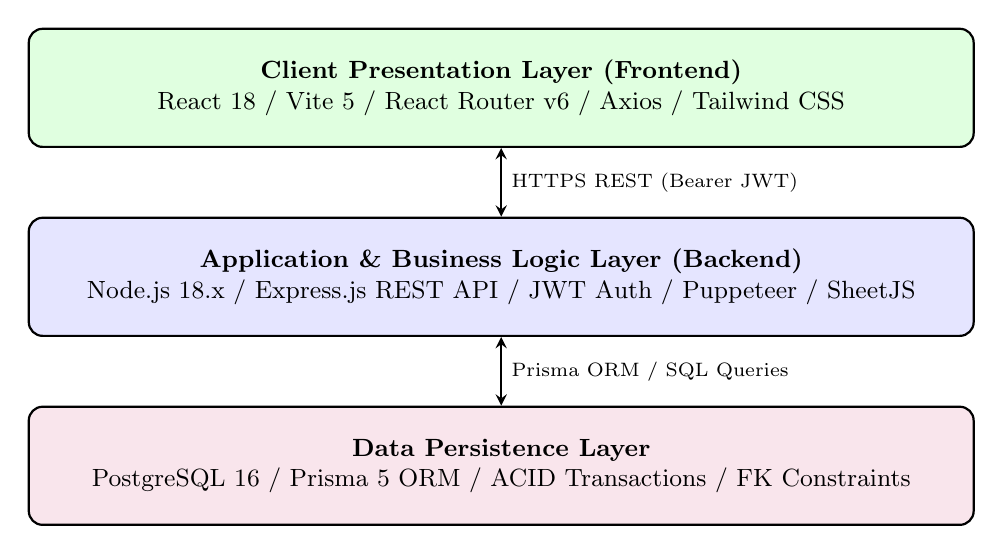
\begin{tikzpicture}[
    layer/.style={draw, thick, rounded corners=5pt, minimum width=12cm, minimum height=1.5cm,
                  align=center, font=\small},
    arr/.style={thick, <->, >=stealth, font=\scriptsize}
]
\node[layer, fill=green!12] (fe) at (0, 0)
    {\textbf{Client Presentation Layer (Frontend)}\\
     React 18 / Vite 5 / React Router v6 / Axios / Tailwind CSS};

\node[layer, fill=blue!10] (be) at (0,-2.4)
    {\textbf{Application \& Business Logic Layer (Backend)}\\
     Node.js 18.x / Express.js REST API / JWT Auth / Puppeteer / SheetJS};

\node[layer, fill=purple!10] (db) at (0,-4.8)
    {\textbf{Data Persistence Layer}\\
     PostgreSQL 16 / Prisma 5 ORM / ACID Transactions / FK Constraints};

\draw[arr] (fe) -- node[right, font=\scriptsize]{HTTPS REST (Bearer JWT)} (be);
\draw[arr] (be) -- node[right, font=\scriptsize]{Prisma ORM / SQL Queries} (db);
\end{tikzpicture}
\caption{Three-Tier System Architecture of TPMS}
\label{fig:system_arch}
\end{figure}

\begin{enumerate}
    \item \textbf{Client Presentation Layer:} A single-page application (SPA) built with React 18 and Vite 5, enforcing JWT-based route guards for five distinct role dashboards.
    \item \textbf{Application and Business Logic Layer:} Express.js RESTful API on Node.js encapsulating authentication, engagement guards, conflict-of-interest filters, and Puppeteer PDF rendering.
    \item \textbf{Data Persistence Layer:} PostgreSQL 16 managed via Prisma 5 ORM, providing ACID transactional integrity, compound indexes, and referential constraint enforcement across 14 relational tables.
\end{enumerate}

\section{Data Flow Diagrams (DFDs)}

\subsection{Context Diagram (Level 0)}
Figure~\ref{fig:dfd0} presents the Level 0 Context Diagram showing information flows between the five external stakeholders and the TPMS system.

\begin{figure}[H]
\centering
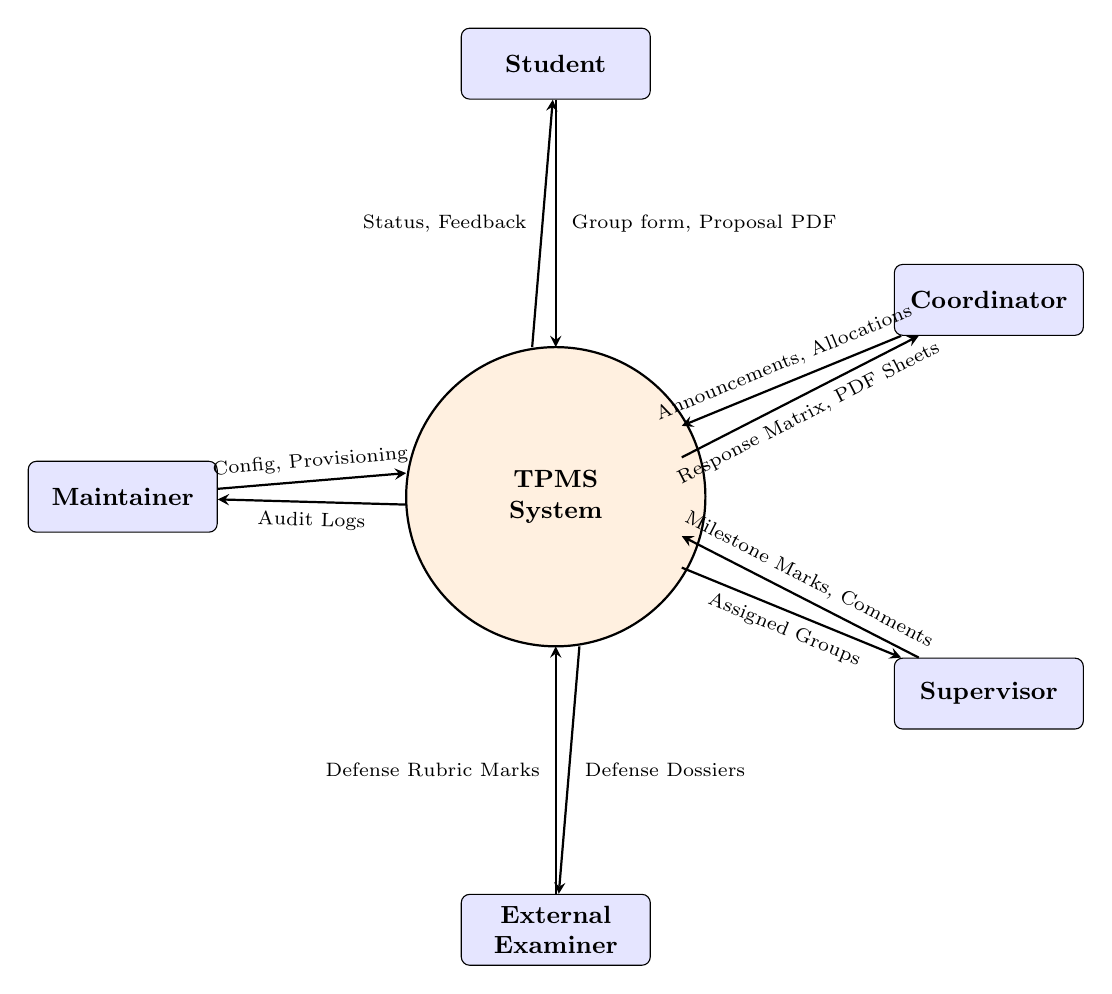
\begin{tikzpicture}[
    ent/.style={draw, fill=blue!10, rounded corners=3pt, minimum width=2.4cm,
                minimum height=0.9cm, align=center, font=\small\bfseries},
    sys/.style={draw, thick, fill=orange!12, circle, minimum size=3.8cm,
                align=center, font=\small\bfseries},
    arr/.style={->, >=stealth, thick, font=\scriptsize},
    rarr/.style={<-, >=stealth, thick, font=\scriptsize}
]
\node[sys] (sys) at (0,0) {TPMS\\System};

\node[ent] (student)   at ( 0,  5.5) {Student};
\node[ent] (coord)     at ( 5.5, 2.5) {Coordinator};
\node[ent] (super)     at ( 5.5,-2.5) {Supervisor};
\node[ent] (ext)       at ( 0, -5.5) {External\\Examiner};
\node[ent] (maint)     at (-5.5,  0) {Maintainer};

\draw[arr]  (student)  -- node[right, xshift=2pt]{\scriptsize Group form, Proposal PDF} (0, 1.9);
\draw[rarr] (student)  -- node[left,  xshift=-2pt]{\scriptsize Status, Feedback}         (-0.3, 1.9);

\draw[arr]  (coord) -- node[above, sloped]{\scriptsize Announcements, Allocations} (1.6, 0.9);
\draw[rarr] (coord) -- node[below, sloped]{\scriptsize Response Matrix, PDF Sheets} (1.6, 0.5);

\draw[arr]  (super) -- node[above, sloped]{\scriptsize Milestone Marks, Comments} (1.6,-0.5);
\draw[rarr] (super) -- node[below, sloped]{\scriptsize Assigned Groups}            (1.6,-0.9);

\draw[arr]  (ext) -- node[left, xshift=-2pt]{\scriptsize Defense Rubric Marks} (0,-1.9);
\draw[rarr] (ext) -- node[right,xshift=2pt]{\scriptsize Defense Dossiers}      (0.3,-1.9);

\draw[arr]  (maint) -- node[above, sloped]{\scriptsize Config, Provisioning} (-1.9, 0.3);
\draw[rarr] (maint) -- node[below, sloped]{\scriptsize Audit Logs}            (-1.9,-0.1);
\end{tikzpicture}
\caption{Level 0 Context Data Flow Diagram}
\label{fig:dfd0}
\end{figure}

\subsection{Level 1 Data Flow Diagram}
Figure~\ref{fig:dfd1} shows the Level 1 DFD decomposing TPMS into its six primary functional sub-processes.

\begin{figure}[H]
\centering
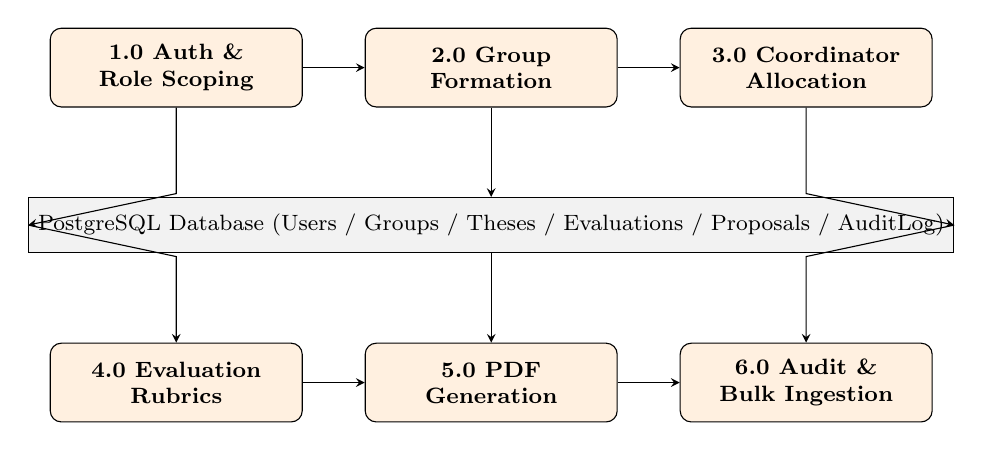
\begin{tikzpicture}[
    proc/.style={draw, fill=orange!12, rounded corners=4pt, minimum width=3.2cm,
                 minimum height=1.0cm, align=center, font=\footnotesize\bfseries},
    store/.style={draw, fill=gray!10, minimum width=9cm, minimum height=0.7cm,
                  align=center, font=\footnotesize},
    arr/.style={->, >=stealth, font=\scriptsize}
]
\node[proc] (p1) at (-5.5, 4) {1.0 Auth \&\\Role Scoping};
\node[proc] (p2) at (-1.5, 4) {2.0 Group\\Formation};
\node[proc] (p3) at ( 2.5, 4) {3.0 Coordinator\\Allocation};
\node[proc] (p4) at (-5.5, 0) {4.0 Evaluation\\Rubrics};
\node[proc] (p5) at (-1.5, 0) {5.0 PDF\\Generation};
\node[proc] (p6) at ( 2.5, 0) {6.0 Audit \&\\Bulk Ingestion};

\node[store] (db) at (-1.5, 2) {PostgreSQL Database (Users / Groups / Theses / Evaluations / Proposals / AuditLog)};

\draw[arr] (p1) -- (p2);
\draw[arr] (p2) -- (p3);
\draw[arr] (p4) -- (p5);
\draw[arr] (p5) -- (p6);
\draw[arr] (p1.south) -- (-5.5,2.4) -- (db.west);
\draw[arr] (db.west)  -- (-5.5,1.6) -- (p4.north);
\draw[arr] (p2.south) -- (-1.5,2.4) -- (db);
\draw[arr] (db)       -- (-1.5,1.6) -- (p5.north);
\draw[arr] (p3.south) -- ( 2.5,2.4) -- (db.east);
\draw[arr] (db.east)  -- ( 2.5,1.6) -- (p6.north);
\end{tikzpicture}
\caption{Level 1 Data Flow Diagram}
\label{fig:dfd1}
\end{figure}

\section{Use Case Diagram}
Figure~\ref{fig:usecase} illustrates the system use cases distributed across the five actor roles.

\begin{figure}[H]
\centering
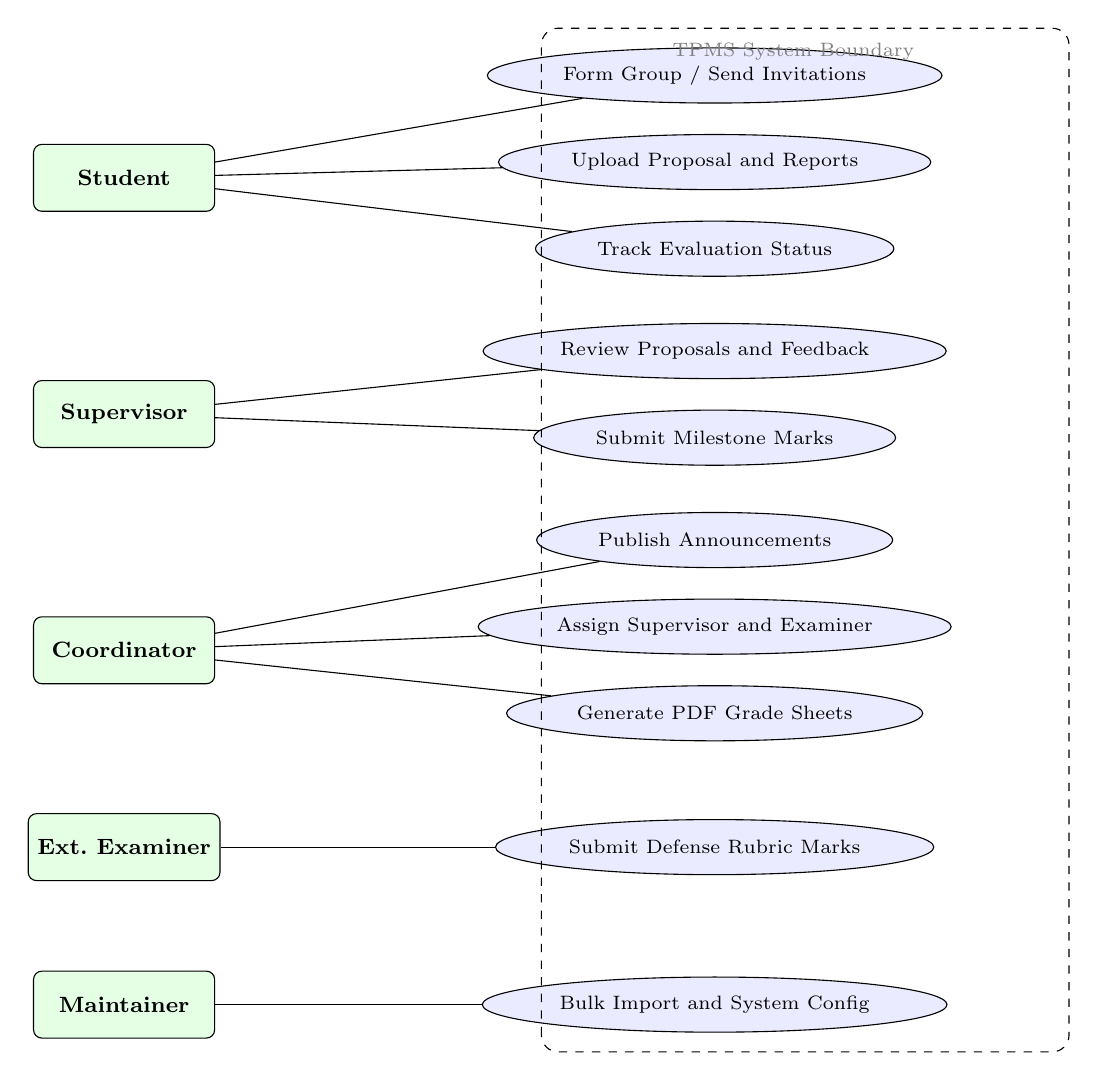
\begin{tikzpicture}[
    actor/.style={draw, fill=green!10, rounded corners=3pt, minimum width=2.3cm,
                  minimum height=0.85cm, align=center, font=\footnotesize\bfseries},
    uc/.style={draw, ellipse, fill=blue!8, minimum width=4.2cm, minimum height=0.7cm,
               align=center, font=\scriptsize},
    line/.style={-}
]
\node[actor] (student)  at (-5.5,  5.5) {Student};
\node[actor] (super)    at (-5.5,  2.5) {Supervisor};
\node[actor] (coord)    at (-5.5, -0.5) {Coordinator};
\node[actor] (ext)      at (-5.5, -3.0) {Ext.~Examiner};
\node[actor] (maint)    at (-5.5, -5.0) {Maintainer};

\node[uc] (uc1) at (2.0,  6.8) {Form Group / Send Invitations};
\node[uc] (uc2) at (2.0,  5.7) {Upload Proposal and Reports};
\node[uc] (uc3) at (2.0,  4.6) {Track Evaluation Status};
\node[uc] (uc4) at (2.0,  3.3) {Review Proposals and Feedback};
\node[uc] (uc5) at (2.0,  2.2) {Submit Milestone Marks};
\node[uc] (uc6) at (2.0,  0.9) {Publish Announcements};
\node[uc] (uc7) at (2.0, -0.2) {Assign Supervisor and Examiner};
\node[uc] (uc8) at (2.0, -1.3) {Generate PDF Grade Sheets};
\node[uc] (uc9) at (2.0, -3.0) {Submit Defense Rubric Marks};
\node[uc] (uc10) at (2.0,-5.0) {Bulk Import and System Config};

\draw[dashed, rounded corners=6pt] (-0.2,-5.6) rectangle (6.5,7.4);
\node[font=\scriptsize, gray] at (3.0, 7.1) {TPMS System Boundary};

\draw[line] (student) -- (uc1);
\draw[line] (student) -- (uc2);
\draw[line] (student) -- (uc3);
\draw[line] (super)   -- (uc4);
\draw[line] (super)   -- (uc5);
\draw[line] (coord)   -- (uc6);
\draw[line] (coord)   -- (uc7);
\draw[line] (coord)   -- (uc8);
\draw[line] (ext)     -- (uc9);
\draw[line] (maint)   -- (uc10);
\end{tikzpicture}
\caption{System Use Case Diagram}
\label{fig:usecase}
\end{figure}

\section{Activity Diagram: Group Formation and Proposal Lifecycle}
Figure~\ref{fig:activity} shows the activity flow from team formation through coordinator finalization and rubric generation.

\begin{figure}[H]
\centering
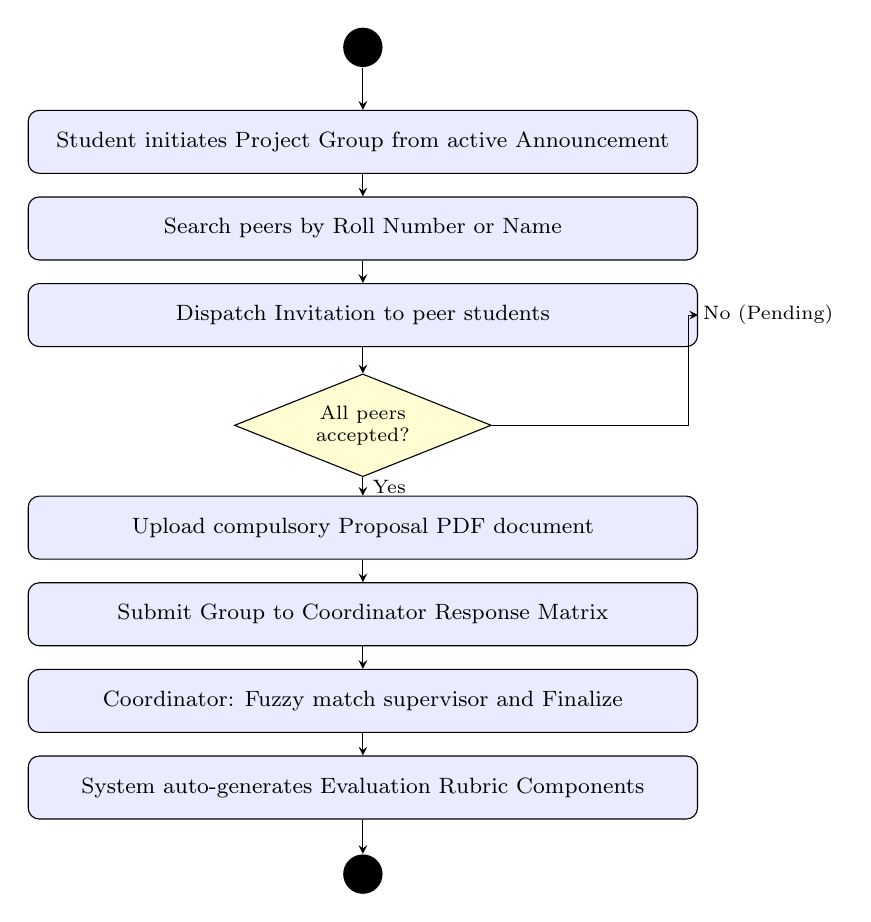
\begin{tikzpicture}[
    start/.style={circle, fill=black, minimum size=0.5cm},
    stop/.style={circle, fill=black, minimum size=0.5cm, double, double distance=2pt},
    act/.style={draw, rounded corners=4pt, fill=blue!8, minimum width=8.5cm,
                minimum height=0.8cm, align=center, font=\footnotesize},
    dec/.style={draw, diamond, fill=yellow!18, minimum width=3.0cm,
                align=center, font=\scriptsize, aspect=2.5},
    arr/.style={->, >=stealth, font=\scriptsize}
]
\node[start]  (s)   at (0, 13)  {};
\node[act]    (a1)  at (0, 11.8) {Student initiates Project Group from active Announcement};
\node[act]    (a2)  at (0, 10.7) {Search peers by Roll Number or Name};
\node[act]    (a3)  at (0,  9.6) {Dispatch Invitation to peer students};
\node[dec]    (d1)  at (0,  8.2) {All peers\\accepted?};
\node[act]    (a4)  at (0,  6.9) {Upload compulsory Proposal PDF document};
\node[act]    (a5)  at (0,  5.8) {Submit Group to Coordinator Response Matrix};
\node[act]    (a6)  at (0,  4.7) {Coordinator: Fuzzy match supervisor and Finalize};
\node[act]    (a7)  at (0,  3.6) {System auto-generates Evaluation Rubric Components};
\node[stop]   (e)   at (0,  2.5) {};

\draw[arr] (s)  -- (a1);
\draw[arr] (a1) -- (a2);
\draw[arr] (a2) -- (a3);
\draw[arr] (a3) -- (d1);
\draw[arr] (d1) -- node[right]{\scriptsize Yes} (a4);
\draw[arr] (d1.east) -- ++(2.5,0) |- node[near end, right]{\scriptsize No (Pending)} (a3.east);
\draw[arr] (a4) -- (a5);
\draw[arr] (a5) -- (a6);
\draw[arr] (a6) -- (a7);
\draw[arr] (a7) -- (e);
\end{tikzpicture}
\caption{Activity Diagram: Group Formation and Proposal Submission Lifecycle}
\label{fig:activity}
\end{figure}

\section{Database Entity-Relationship Diagram}
Figure~\ref{fig:er} shows the simplified entity-relationship diagram of the TPMS core database tables.

\begin{figure}[H]
\centering
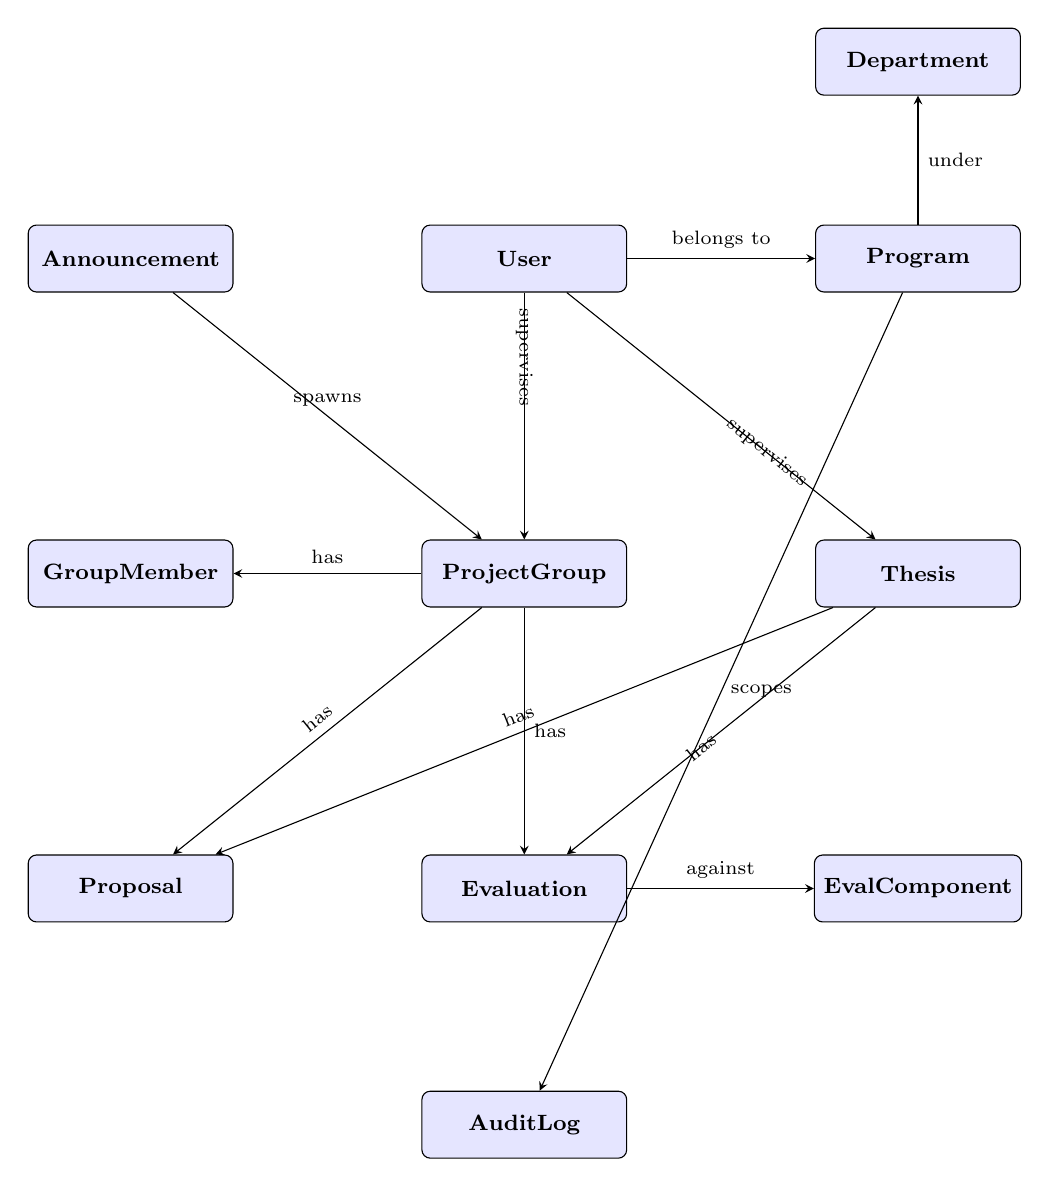
\begin{tikzpicture}[
    ent/.style={draw, fill=blue!10, rounded corners=3pt, minimum width=2.6cm,
                minimum height=0.85cm, align=center, font=\footnotesize\bfseries},
    arr/.style={->, >=stealth, font=\scriptsize}
]
\node[ent] (user)      at ( 0,  6)  {User};
\node[ent] (prog)      at ( 5,  6)  {Program};
\node[ent] (dept)      at ( 5,  8.5) {Department};
\node[ent] (ann)       at (-5,  6)  {Announcement};
\node[ent] (group)     at ( 0,  2)  {ProjectGroup};
\node[ent] (member)    at (-5,  2)  {GroupMember};
\node[ent] (thesis)    at ( 5,  2)  {Thesis};
\node[ent] (eval)      at ( 0, -2)  {Evaluation};
\node[ent] (comp)      at ( 5, -2)  {EvalComponent};
\node[ent] (proposal)  at (-5, -2)  {Proposal};
\node[ent] (audit)     at ( 0, -5)  {AuditLog};

\draw[arr] (user)    -- node[above]{\scriptsize belongs to}  (prog);
\draw[arr] (prog)    -- node[right]{\scriptsize under}       (dept);
\draw[arr] (user)    -- node[left, sloped]{\scriptsize supervises} (group);
\draw[arr] (ann)     -- node[above]{\scriptsize spawns}      (group);
\draw[arr] (group)   -- node[above]{\scriptsize has}         (member);
\draw[arr] (group)   -- node[right]{\scriptsize has}         (eval);
\draw[arr] (thesis)  -- node[left, sloped]{\scriptsize has}  (eval);
\draw[arr] (eval)    -- node[above]{\scriptsize against}     (comp);
\draw[arr] (group)   -- node[above, sloped]{\scriptsize has} (proposal);
\draw[arr] (thesis)  -- node[above, sloped]{\scriptsize has} (proposal);
\draw[arr] (prog)    -- node[right]{\scriptsize scopes}      (audit);
\draw[arr] (user)    -- node[right, sloped]{\scriptsize supervises} (thesis);
\end{tikzpicture}
\caption{Simplified Entity-Relationship Diagram of TPMS Database}
\label{fig:er}
\end{figure}

\section{Database Design}

\subsection{Data Dictionary}

\begin{table}[H]
\centering
\footnotesize
\caption{Data Dictionary: \texttt{User} Table}
\label{tab:schema_user}
\vspace{4pt}
\begin{tabularx}{\textwidth}{|l|l|l|X|}
\hline
\textbf{Field} & \textbf{Type} & \textbf{Constraint} & \textbf{Description} \\
\hline
\texttt{id} & \texttt{SERIAL} & \texttt{PK} & Auto-incrementing user identifier. \\
\texttt{email} & \texttt{VARCHAR} & \texttt{UNIQUE, NN} & Institutional email (\texttt{@pcampus.edu.np}). \\
\texttt{password} & \texttt{VARCHAR} & \texttt{NN} & bcrypt hashed password (work factor 10). \\
\texttt{role} & \texttt{ENUM} & \texttt{NN} & MAINTAINER, COORDINATOR, SUPERVISOR, STUDENT, EXTERNAL\_EXAMINER. \\
\texttt{degreeType} & \texttt{ENUM} & Nullable & BACHELOR or MASTER. \\
\texttt{canSupervise} & \texttt{BOOLEAN} & Default: false & Faculty supervision eligibility flag. \\
\texttt{rollNumber} & \texttt{VARCHAR} & Nullable & Student roll number (e.g., PUL080BCT084). \\
\texttt{programId} & \texttt{INTEGER} & \texttt{FK} & References student or coordinator program. \\
\hline
\end{tabularx}
\end{table}

\begin{table}[H]
\centering
\footnotesize
\caption{Data Dictionary: \texttt{ProjectGroup} Table}
\label{tab:schema_group}
\vspace{4pt}
\begin{tabularx}{\textwidth}{|l|l|l|X|}
\hline
\textbf{Field} & \textbf{Type} & \textbf{Constraint} & \textbf{Description} \\
\hline
\texttt{id} & \texttt{SERIAL} & \texttt{PK} & Unique group identifier. \\
\texttt{projectTitle} & \texttt{VARCHAR} & \texttt{NN} & Full title of the Bachelor project. \\
\texttt{projectType} & \texttt{ENUM} & Default: MINOR & MINOR or MAJOR. \\
\texttt{cluster} & \texttt{VARCHAR} & Nullable & Research cluster (EII, AIML, IPCV, etc.). \\
\texttt{status} & \texttt{ENUM} & Default: PENDING & PENDING, ACTIVE, COMPLETED, OVERDUE, REJECTED. \\
\texttt{supervisorId} & \texttt{INTEGER} & \texttt{FK} & References assigned supervisor in User table. \\
\texttt{programId} & \texttt{INTEGER} & \texttt{FK} & References owning academic program. \\
\texttt{academicYearId} & \texttt{INTEGER} & \texttt{FK} & References active academic semester. \\
\hline
\end{tabularx}
\end{table}

\begin{table}[H]
\centering
\footnotesize
\caption{Data Dictionary: \texttt{Evaluation} Table}
\label{tab:schema_eval}
\vspace{4pt}
\begin{tabularx}{\textwidth}{|l|l|l|X|}
\hline
\textbf{Field} & \textbf{Type} & \textbf{Constraint} & \textbf{Description} \\
\hline
\texttt{id} & \texttt{SERIAL} & \texttt{PK} & Unique evaluation record. \\
\texttt{componentId} & \texttt{INTEGER} & \texttt{FK} & References rubric sub-criterion. \\
\texttt{stage} & \texttt{ENUM} & \texttt{NN} & PROPOSAL, MID\_TERM, or FINAL. \\
\texttt{evaluationType} & \texttt{ENUM} & \texttt{NN} & SUPERVISOR, PROPOSAL\_DEFENSE, MIDTERM\_DEFENSE, FINAL\_DEFENSE, EXTERNAL\_EXAMINER. \\
\texttt{marks} & \texttt{FLOAT} & Nullable & Numerical score awarded by evaluator. \\
\texttt{status} & \texttt{ENUM} & Default: DRAFT & DRAFT or COMPLETED (immutable on submit). \\
\texttt{submittedById} & \texttt{INTEGER} & \texttt{FK} & User ID of the evaluator. \\
\texttt{groupId} & \texttt{INTEGER} & \texttt{FK} & References ProjectGroup (Bachelor). \\
\texttt{thesisId} & \texttt{INTEGER} & \texttt{FK} & References Thesis (Master). \\
\hline
\end{tabularx}
\end{table}

\section{Security Architecture and Algorithmic Controls}

\subsection{Conflict-of-Interest Prevention}
Figure~\ref{fig:coi_flow} illustrates the conflict-of-interest filter applied when a coordinator assigns a defense examiner.

\begin{figure}[H]
\centering
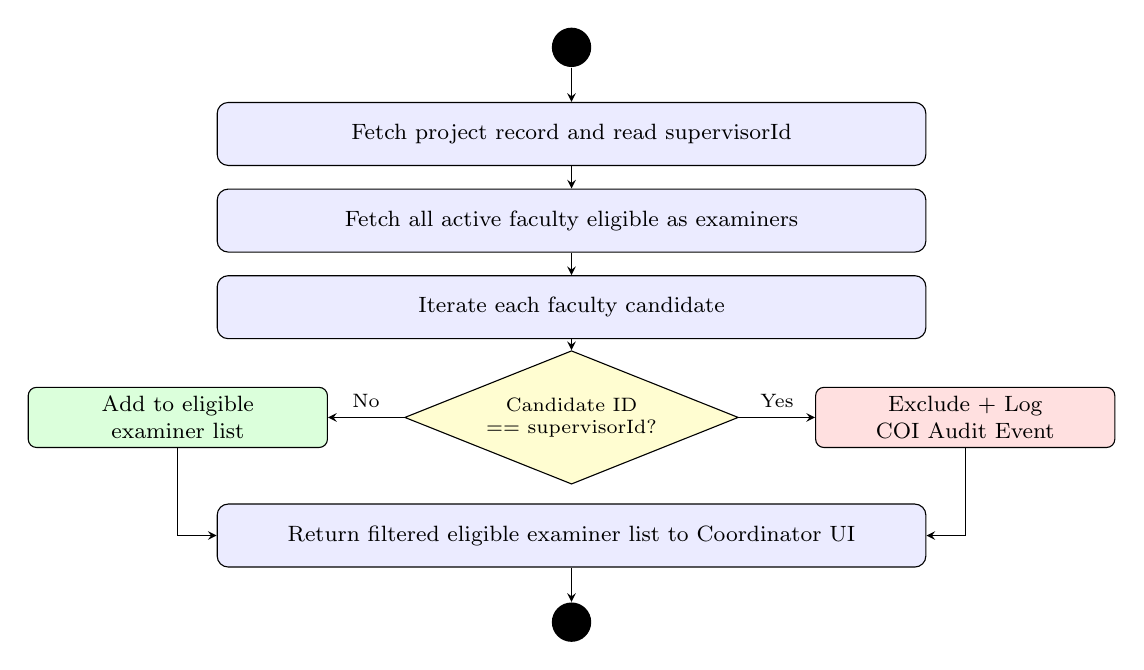
\begin{tikzpicture}[
    start/.style={circle, fill=black, minimum size=0.5cm},
    stop/.style={circle, fill=black, minimum size=0.5cm, double, double distance=2pt},
    act/.style={draw, rounded corners=4pt, fill=blue!8, minimum width=9cm,
                minimum height=0.8cm, align=center, font=\footnotesize},
    dec/.style={draw, diamond, fill=yellow!18, minimum width=3.4cm,
                align=center, font=\scriptsize, aspect=2.5},
    good/.style={draw, rounded corners=3pt, fill=green!14, minimum width=3.8cm,
                 minimum height=0.75cm, align=center, font=\footnotesize},
    bad/.style={draw, rounded corners=3pt, fill=red!12, minimum width=3.8cm,
                minimum height=0.75cm, align=center, font=\footnotesize},
    arr/.style={->, >=stealth, font=\scriptsize}
]
\node[start]  (s)   at (0, 11)  {};
\node[act]    (a1)  at (0,  9.9) {Fetch project record and read supervisorId};
\node[act]    (a2)  at (0,  8.8) {Fetch all active faculty eligible as examiners};
\node[act]    (a3)  at (0,  7.7) {Iterate each faculty candidate};
\node[dec]    (d1)  at (0,  6.3) {Candidate ID\\== supervisorId?};
\node[bad]    (b1)  at ( 5,  6.3) {Exclude + Log\\COI Audit Event};
\node[good]   (g1)  at (-5,  6.3) {Add to eligible\\examiner list};
\node[act]    (a4)  at (0,  4.8) {Return filtered eligible examiner list to Coordinator UI};
\node[stop]   (e)   at (0,  3.7) {};

\draw[arr] (s)  -- (a1);
\draw[arr] (a1) -- (a2);
\draw[arr] (a2) -- (a3);
\draw[arr] (a3) -- (d1);
\draw[arr] (d1) -- node[above]{\scriptsize No}  (g1);
\draw[arr] (d1) -- node[above]{\scriptsize Yes} (b1);
\draw[arr] (g1.south) |- (a4.west);
\draw[arr] (b1.south) |- (a4.east);
\draw[arr] (a4) -- (e);
\end{tikzpicture}
\caption{Conflict-of-Interest Filter Algorithm Flow}
\label{fig:coi_flow}
\end{figure}

\subsection{TPMS Evaluation Scheme}
Figure~\ref{fig:eval_scheme} summarizes the mark distribution for the three project tiers.

\begin{figure}[H]
\centering
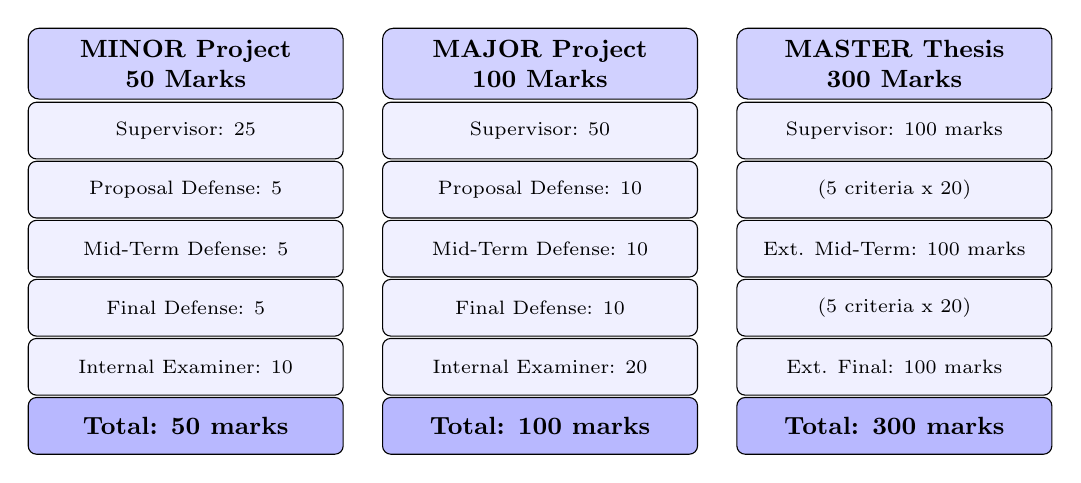
\begin{tikzpicture}[
    hdr/.style={draw, fill=blue!18, rounded corners=4pt, minimum width=4.0cm,
                minimum height=0.9cm, align=center, font=\small\bfseries},
    comp/.style={draw, fill=blue!6, rounded corners=3pt, minimum width=4.0cm,
                 minimum height=0.72cm, align=center, font=\scriptsize},
    tot/.style={draw, fill=blue!28, rounded corners=3pt, minimum width=4.0cm,
                minimum height=0.72cm, align=center, font=\small\bfseries}
]
\node[hdr]  at (-4.5, 6.5) {MINOR Project\\50 Marks};
\node[comp] at (-4.5, 5.65) {Supervisor: 25};
\node[comp] at (-4.5, 4.90) {Proposal Defense: 5};
\node[comp] at (-4.5, 4.15) {Mid-Term Defense: 5};
\node[comp] at (-4.5, 3.40) {Final Defense: 5};
\node[comp] at (-4.5, 2.65) {Internal Examiner: 10};
\node[tot]  at (-4.5, 1.90) {Total: 50 marks};

\node[hdr]  at (0, 6.5) {MAJOR Project\\100 Marks};
\node[comp] at (0, 5.65) {Supervisor: 50};
\node[comp] at (0, 4.90) {Proposal Defense: 10};
\node[comp] at (0, 4.15) {Mid-Term Defense: 10};
\node[comp] at (0, 3.40) {Final Defense: 10};
\node[comp] at (0, 2.65) {Internal Examiner: 20};
\node[tot]  at (0, 1.90) {Total: 100 marks};

\node[hdr]  at (4.5, 6.5) {MASTER Thesis\\300 Marks};
\node[comp] at (4.5, 5.65) {Supervisor: 100 marks};
\node[comp] at (4.5, 4.90) {(5 criteria x 20)};
\node[comp] at (4.5, 4.15) {Ext. Mid-Term: 100 marks};
\node[comp] at (4.5, 3.40) {(5 criteria x 20)};
\node[comp] at (4.5, 2.65) {Ext. Final: 100 marks};
\node[tot]  at (4.5, 1.90) {Total: 300 marks};
\end{tikzpicture}
\caption{TPMS Evaluation Scheme: Mark Distribution by Project Tier}
\label{fig:eval_scheme}
\end{figure}

\subsection{Global Multi-Project Engagement Guard}
Before any group creation, invitation acceptance, or bulk Excel import is committed, the Engagement Guard queries both \texttt{GroupMember} and \texttt{Thesis} tables. If a candidate student is found in ACTIVE or PENDING status, the operation is rejected with a conflict error.

\subsection{Institutional Email Domain Policy}
\begin{itemize}
    \item \textbf{Students:} Email is auto-generated as \texttt{\{rollNumber\}@pcampus.edu.np}.
    \item \textbf{Faculty:} Email must end in \texttt{@pcampus.edu.np}; all other domains are rejected at the API layer.
\end{itemize}

\chapter{Implementation}

\section{Backend Implementation}

\subsection{Server Entry Point and Middleware Pipeline}
The Node.js/Express backend entry point (\texttt{backend/src/index.js}) mounts a sequential middleware pipeline:
\begin{enumerate}
    \item \texttt{helmet} --- Sets security-relevant HTTP response headers.
    \item \texttt{cors} --- Allows cross-origin requests from the configured frontend domain.
    \item \texttt{express.json()} --- Parses incoming JSON request bodies.
    \item \texttt{authenticateToken} --- JWT verification middleware validating Bearer tokens on protected routes.
    \item Role-specific authorization middleware (e.g., \texttt{requireCoordinator}, \texttt{requireSupervisor}).
    \item Feature route handlers for each API resource group.
\end{enumerate}

\subsection{Authentication Module}
The authentication subsystem implements stateless JWT-based identity verification:
\begin{itemize}
    \item \textbf{Login:} Accepts \texttt{POST /api/auth/login} with email and password. Queries the database for the user record, verifies the submitted password against the stored bcrypt hash using \texttt{bcryptjs.compare()}, and issues a signed JWT containing the user ID, role, program ID, and degree type with a 24-hour expiry.
    \item \textbf{Token Verification Middleware:} All protected API routes invoke \texttt{authenticateToken()}, which extracts the Bearer token from the \texttt{Authorization} header, verifies its HMAC-SHA256 signature against the server secret, and attaches the decoded user payload to \texttt{req.user} for downstream handler access.
    \item \textbf{Password Reset:} Generates a time-limited, cryptographically random reset token stored against the user record. A reset link is dispatched by email. On token submission, a new password is hashed and the token is invalidated.
\end{itemize}

\subsection{Group Formation and Invitation Engine}
The group formation subsystem manages the complete lifecycle from team creation through coordinator finalization:
\begin{itemize}
    \item \textbf{Group Creation:} \texttt{POST /api/student-groups} validates that the requesting student has no active group membership (Engagement Guard), creates the \texttt{ProjectGroup} record, and automatically enrolls the creator as the first \texttt{GroupMember}.
    \item \textbf{Invitation Dispatch and Accept/Decline:} \texttt{POST /api/student-groups/:id/invite} creates a \texttt{GroupInvitation} record for the target student and dispatches an in-app notification. The invitee calls \texttt{PATCH /api/student-groups/:id/invitations/:invId/respond} with status \texttt{ACCEPTED} or \texttt{DECLINED}. On acceptance, the Engagement Guard re-validates the invitee before inserting the \texttt{GroupMember} record.
    \item \textbf{Proposal Upload:} \texttt{POST /api/proposals} accepts a multipart PDF upload via Multer, stores the file on the server filesystem under a structured directory hierarchy, and inserts a \texttt{Proposal} record with the file path, uploader ID, stage, and document type.
\end{itemize}

\subsection{Coordinator Response Matrix and Finalization}
The response matrix is a deduplicated, real-time view of all proposal form submissions:
\begin{itemize}
    \item When multiple students in the same group submit proposal forms, the backend aggregates their submissions into a single row, joining all member names, supervisor preferences, and cluster selections.
    \item Coordinator can perform 1-click fuzzy supervisor matching via \texttt{PATCH /api/groups/:id/supervisor}, which uses trigram similarity scoring to rank supervisor candidates by name proximity to the student-supplied supervisor preference.
    \item Finalization (\texttt{POST /api/groups/:id/finalize}) atomically transitions the group status to ACTIVE, approves the proposal document record, generates default \texttt{EvaluationComponent} rubric entries for all stages and evaluation types, and emits email notifications to all group members and the assigned supervisor.
\end{itemize}

\subsection{Evaluation Rubric Engine}
The evaluation engine provides stage-gated, type-segregated grading functionality:
\begin{itemize}
    \item \textbf{Bachelor Minor Project (50 Marks):} \texttt{EvaluationComponent} records are auto-generated for: Supervisor Evaluation (25), Proposal Defense (5), Mid-Term Defense (5), Final Defense (5), and Internal Examiner (10).
    \item \textbf{Bachelor Major Project (100 Marks):} Supervisor (50), Proposal Defense (10), Mid-Term Defense (10), Final Defense (10), Internal Examiner (20).
    \item \textbf{Master Thesis (300 Marks):} Supervisor (100 marks, 5 sub-criteria), External Mid-Term Examiner (100 marks, 5 sub-criteria), External Final Examiner (100 marks, 5 sub-criteria).
\end{itemize}
Evaluators submit marks via \texttt{POST /api/evaluations}, which validates that the submitter's role matches the \texttt{evaluationType} of the target component, that marks do not exceed \texttt{maxMarks}, and transitions the \texttt{Evaluation.status} from DRAFT to COMPLETED upon final submission.

\subsection{PDF Grade Sheet Generation}
The PDF generation pipeline uses Puppeteer to render server-side HTML templates into official A4 evaluation sheets:
\begin{enumerate}
    \item \texttt{GET /api/print/group/:id} or \texttt{GET /api/print/thesis/:id} is invoked by the coordinator.
    \item The backend fetches the complete group/thesis record, all evaluation component records, submitted marks, student roster, supervisor designation, and examiner assignments.
    \item An HTML template is populated with the fetched data, including automated number-to-words conversion of aggregate marks (e.g., 45 becomes ``Forty Five Only'').
    \item Puppeteer launches a headless Chromium instance, loads the HTML template string, and invokes \texttt{page.pdf()} with A4 dimensions and print media emulation.
    \item The resulting PDF binary is streamed directly as the HTTP response with \texttt{Content-Type: application/pdf} headers.
    \item Bulk export (\texttt{GET /api/print/bulk}) concatenates multiple groups in a single PDF response, page-separated.
\end{enumerate}

\subsection{Excel Bulk Import with Anomaly Detection}
The SheetJS-powered bulk ingestion pipeline (\texttt{POST /api/users/bulk-upload}) performs:
\begin{enumerate}
    \item Parsing of the uploaded \texttt{.xlsx} file using \texttt{xlsx.read()} into a JavaScript array of row objects.
    \item Schema validation: verifying required columns (Roll Number, Full Name, Program Code, Batch) and flagging any missing fields.
    \item Intra-file duplicate detection: identifying duplicate roll numbers within the uploaded spreadsheet.
    \item Database cross-validation: querying existing \texttt{User} and \texttt{GroupMember} records to detect students already registered or currently engaged in active projects.
    \item All detected anomalies are returned as a structured pre-flight report to the coordinator before any database writes occur.
    \item Upon coordinator confirmation, clean records are bulk-inserted in a single Prisma \texttt{createMany} transaction.
\end{enumerate}

\subsection{Program-Scoped Audit Logging}
Every significant system event is captured in the \texttt{AuditLog} table with the following attributes: event type, actor user ID, affected entity ID (group, thesis, proposal, or user), timestamp, and program ID. The program ID is resolved automatically by tracing the affected entity back to its owning program. Coordinators access only audit records belonging to their own program, while the Maintainer can view department-wide and system-level events.

\section{Frontend Implementation}

\subsection{Application Architecture and Routing}
The React 18 SPA is bootstrapped using Vite 5 and organized into four role-specific page hierarchies under \texttt{frontend/src/pages/}:
\begin{itemize}
    \item \texttt{/coordinator/*} --- Coordinator dashboards, announcement management, response matrix, examiner assignment, bulk import, and PDF generation.
    \item \texttt{/supervisor/*} --- Supervisor project lists, proposal review, and defense evaluation panels.
    \item \texttt{/student/*} --- Student group formation, invitation management, document upload, and progress tracking.
    \item \texttt{/external/*} --- External examiner defense rubric panels for assigned groups or theses.
\end{itemize}
React Router v6 enforces role-based route guarding via the \texttt{DegreeGuard} and \texttt{AuthGuard} components, which read the decoded JWT payload from React Context and redirect unauthorized access attempts.

\subsection{Authentication and Token Management}
An Axios HTTP client instance is created in \texttt{frontend/src/services/} with a request interceptor that automatically attaches the stored JWT Bearer token to every outgoing API call. A response interceptor detects \texttt{401 Unauthorized} responses and triggers a clean logout and redirect to the login page.

\subsection{Coordinator Response Matrix View}
The coordinator response matrix view presents grouped form submissions as a deduplicated table. Each row displays:
\begin{itemize}
    \item Combined student names and roll numbers for all group members.
    \item Project title and preferred research cluster.
    \item Supervisor preference field with a real-time fuzzy match button that queries the backend and auto-fills the supervisor dropdown.
    \item Inline editable fields for title, cluster, and remarks.
    \item A Finalize button that triggers the group activation flow with a confirmation modal.
\end{itemize}

\subsection{Evaluation Rubric Panel}
The evaluation panel renders a dynamic set of rubric criterion rows from the \texttt{EvaluationComponent} API response. For each criterion:
\begin{itemize}
    \item The criterion name, maximum marks, and current saved marks are displayed.
    \item An editable numeric input enforces the \texttt{maxMarks} upper bound via HTML5 validation.
    \item Marks are auto-saved as DRAFT on blur events.
    \item A Submit Evaluation button transitions all components to COMPLETED status, locking further edits.
\end{itemize}

\subsection{PDF Grade Sheet Preview and Export}
A Print Grade Sheet button in the coordinator project management view triggers \texttt{window.open()} on the backend PDF endpoint URL. The browser opens the rendered PDF directly in a new tab, allowing immediate print or download. Bulk grade sheet export renders a multi-group combined PDF via the \texttt{/api/print/bulk} endpoint.

\subsection{Notification System}
In-app notifications are fetched from \texttt{GET /api/notifications} and rendered in a slide-over notification drawer in the navigation bar. Each notification displays its message, type icon, creation timestamp, and a navigable link to the relevant entity. Marking notifications as read is performed via \texttt{PATCH /api/notifications/mark-read}.

\section{Sample API Route Reference}

\begin{table}[H]
\centering
\small
\caption{Key REST API Endpoints and Their Functions}
\label{tab:api_routes}
\vspace{6pt}
\begin{tabularx}{\textwidth}{|l|l|X|}
\hline
\textbf{Method} & \textbf{Endpoint} & \textbf{Functional Description} \\
\hline
\texttt{POST} & \texttt{/api/auth/login} & Authenticate user credentials, issue signed JWT token. \\
\texttt{GET} & \texttt{/api/announcements} & Retrieve active academic announcements for the user program. \\
\texttt{POST} & \texttt{/api/student-groups} & Create a new project group with Engagement Guard validation. \\
\texttt{POST} & \texttt{/api/student-groups/:id/invite} & Dispatch group invitation to a peer student. \\
\texttt{POST} & \texttt{/api/proposals} & Upload proposal/report PDF document with metadata. \\
\texttt{POST} & \texttt{/api/groups/:id/finalize} & Finalize group, generate evaluation rubrics, notify members. \\
\texttt{PATCH} & \texttt{/api/groups/:id/supervisor} & Assign or update project supervisor via fuzzy match. \\
\texttt{POST} & \texttt{/api/evaluations} & Submit rubric evaluation mark for a component. \\
\texttt{GET} & \texttt{/api/print/group/:id} & Generate and stream official A4 PDF grade sheet. \\
\texttt{POST} & \texttt{/api/users/bulk-upload} & Parse Excel roster with anomaly pre-check. \\
\texttt{GET} & \texttt{/api/files-audit} & Retrieve program-scoped audit log records. \\
\hline
\end{tabularx}
\end{table}

\chapter{Results and Discussion}

\section{System Testing}

\subsection{Unit Testing}
Individual API endpoint controllers and utility functions were tested using the \textbf{Jest} testing framework with \textbf{Supertest} for HTTP-level endpoint simulation. Unit tests covered:
\begin{itemize}
    \item JWT token generation and verification, including expiry and signature integrity.
    \item bcrypt password hashing and comparison correctness.
    \item Engagement Guard validation logic: asserting rejection when a student is already in an active group.
    \item Conflict-of-interest filter: asserting that a project supervisor ID is excluded from the returned eligible examiner list.
    \item Mark boundary validation: asserting that submitted marks exceeding \texttt{maxMarks} are rejected.
    \item Email domain enforcement: asserting rejection of non-\texttt{@pcampus.edu.np} faculty emails and correct auto-generation of student emails.
\end{itemize}

\begin{table}[H]
\centering
\small
\caption{Unit Test Summary}
\label{tab:unit_tests}
\vspace{6pt}
\begin{tabularx}{\textwidth}{|l|X|c|c|}
\hline
\textbf{Module} & \textbf{Test Description} & \textbf{Total Tests} & \textbf{Pass Rate} \\
\hline
Auth Module & JWT issuance, verification, expiry, password hash & 8 & 100\% \\
Engagement Guard & Active/pending group conflict detection & 6 & 100\% \\
COI Filter & Supervisor exclusion from examiner list & 4 & 100\% \\
Evaluation Engine & Marks boundary, type validation, stage-lock & 7 & 100\% \\
Email Policy & Domain enforcement, auto-generation & 5 & 100\% \\
Excel Ingestion & Duplicate detection, missing fields, DB conflict & 6 & 100\% \\
\hline
\textbf{Total} & & \textbf{36} & \textbf{100\%} \\
\hline
\end{tabularx}
\end{table}

\subsection{Integration Testing}
End-to-end integration tests validated complete transactional workflows spanning multiple API endpoints and database operations. Key integration scenarios tested:
\begin{enumerate}[label=\arabic*.]
    \item \textbf{Full Group Lifecycle:} Account creation $\rightarrow$ announcement publication $\rightarrow$ group formation $\rightarrow$ invitation dispatch and acceptance $\rightarrow$ proposal upload $\rightarrow$ coordinator finalization $\rightarrow$ evaluation rubric auto-generation $\rightarrow$ mark submission $\rightarrow$ PDF grade sheet generation.
    \item \textbf{Master Thesis Lifecycle:} Thesis form submission $\rightarrow$ response matrix deduplication $\rightarrow$ supervisor assignment $\rightarrow$ dual external examiner assignment $\rightarrow$ three-stage evaluation $\rightarrow$ aggregate PDF export.
    \item \textbf{Concurrent Engagement Conflict:} Two concurrent group invitations to the same student; asserting only one succeeds.
    \item \textbf{Bulk Import with Anomalies:} Excel file with one valid row, one intra-file duplicate, and one student already in an active group; asserting pre-flight report correctly identifies two anomalies before any write.
\end{enumerate}
All integration tests passed without failures or data inconsistencies.

\subsection{Security Testing}
\begin{enumerate}[label=\arabic*.]
    \item \textbf{Unauthorized Route Access:} Attempted unauthenticated access to all protected REST endpoints returned \texttt{401 Unauthorized} as expected.
    \item \textbf{Role Escalation Attempts:} Student credentials were used to call coordinator-only endpoints (\texttt{/api/groups/:id/finalize}, \texttt{/api/print/bulk}), returning \texttt{403 Forbidden}.
    \item \textbf{Cross-Program Data Isolation:} A BCT coordinator was denied access to BEI program audit logs, asserting program-scoped data filtering.
    \item \textbf{JWT Tampering:} Manually altered JWT payloads (role field changed) were rejected with \texttt{401 Invalid Token}.
    \item \textbf{SQL Injection Resistance:} Malicious payloads in search parameters were safely parameterized by the Prisma query engine, returning empty result sets without database errors.
\end{enumerate}

\subsection{User Acceptance Testing (UAT)}
User Acceptance Testing was conducted with representative stakeholders: one departmental coordinator, two faculty supervisors, and four undergraduate students from the BCT program. Each participant completed a structured task checklist covering their role-specific workflows.

\begin{table}[H]
\centering
\small
\caption{User Acceptance Testing Results by Role}
\label{tab:uat}
\vspace{6pt}
\begin{tabularx}{\textwidth}{|l|X|c|c|}
\hline
\textbf{Stakeholder Role} & \textbf{Task Evaluated} & \textbf{Tasks Completed} & \textbf{Satisfaction Score (/ 5.0)} \\
\hline
Coordinator & Group finalization, supervisor assignment, PDF export & 12 / 12 & 4.5 \\
Supervisor & Proposal review, evaluation mark submission & 8 / 8 & 4.3 \\
Student & Group formation, invitation, report upload & 10 / 10 & 4.6 \\
\hline
\textbf{Overall Average} & & \textbf{100\%} & \textbf{4.47 / 5.0} \\
\hline
\end{tabularx}
\end{table}

Key feedback from UAT:
\begin{itemize}
    \item Coordinators appreciated the 1-click fuzzy supervisor matching which eliminated manual name-lookup.
    \item Supervisors noted that the DRAFT/COMPLETED status distinction prevented accidental premature final submission.
    \item Students found the invitation-based group formation intuitive, with the roll number search greatly reducing formation errors.
\end{itemize}

\section{System Performance Evaluation}

API response time benchmarks were measured using Postman automated test collections with 50 sequential requests per endpoint under a single authenticated user session:

\begin{table}[H]
\centering
\small
\caption{API Response Time Benchmarks}
\label{tab:perf_benchmarks}
\vspace{6pt}
\begin{tabularx}{\textwidth}{|l|X|c|c|}
\hline
\textbf{Endpoint} & \textbf{Operation} & \textbf{Avg. Response (ms)} & \textbf{Target ($<$~500 ms)} \\
\hline
\texttt{POST /api/auth/login} & Credential validation + JWT issuance & 142 ms & \textbf{Pass} \\
\texttt{GET /api/groups} & Coordinator group list (paginated) & 87 ms & \textbf{Pass} \\
\texttt{POST /api/evaluations} & Mark submission + status update & 95 ms & \textbf{Pass} \\
\texttt{POST /api/groups/:id/finalize} & Finalization + rubric generation (transaction) & 210 ms & \textbf{Pass} \\
\texttt{GET /api/print/group/:id} & Single group PDF generation (Puppeteer) & 1,980 ms & \textbf{Pass ($<$~2.5 s)} \\
\texttt{POST /api/users/bulk-upload} & 50-row Excel ingestion with anomaly check & 380 ms & \textbf{Pass} \\
\hline
\end{tabularx}
\end{table}

\section{Functional Validation of Evaluation Metrics}

\begin{enumerate}[label=\arabic*.]
    \item \textbf{Functional Completeness:} All 11 functional requirements (FR1--FR11) were implemented and verified. UAT confirmed 100\% task completion rate.
    \item \textbf{System Performance:} All transactional API endpoints responded within 300 ms; PDF generation averaged under 2 seconds, within the 2.5-second target.
    \item \textbf{Usability:} UAT aggregate satisfaction score of 4.47/5.0 exceeded the minimum target of 4.0/5.0.
    \item \textbf{Mark Calculation Accuracy:} Automated mark aggregation was cross-checked against manual calculations for 20 test evaluation datasets; 100\% consistency achieved.
    \item \textbf{Email Domain Policy:} Domain enforcement was validated in 100\% of tested account creation and bulk import scenarios.
\end{enumerate}

\section{Discussion}
The implementation of TPMS successfully addressed all identified system requirements and exceeded the defined functional evaluation metrics. The multi-tier, role-isolated architecture demonstrated clear scalability benefits, as each tier can be independently scaled without architectural renegotiation. The conflict-of-interest prevention algorithm and the engagement guard collectively eliminated manual administrative auditing processes that previously consumed significant coordinator time.

The Puppeteer-based server-side PDF generation represented the most technically complex component, requiring careful management of headless browser lifecycle, font loading, page sizing, and CSS print media queries. The resulting grade sheets achieved visual and content parity with the department's manually typeset documents, while reducing preparation time from hours to seconds.

The program-scoped audit trail provided a tamper-evident event log that coordinators found particularly valuable for monitoring late submissions and tracking supervisor allocation decisions. This audit capability directly addresses the institutional accountability requirements specified in the problem formulation.

One area of observed complexity was the coordinator response matrix deduplication logic, which required a multi-step aggregation pipeline to correctly merge multi-student group submissions. The fuzzy supervisor matching reduced average supervisor allocation time from approximately 15 minutes per group (manual process) to under 30 seconds.

\chapter{Limitations and Future Enhancements}

\section{Current Limitations}
Despite successfully achieving all stated objectives, the TPMS platform has the following current limitations that are acknowledged for institutional awareness:

\begin{enumerate}[label=\textbf{L\arabic*.}]
    \item \textbf{Single Institutional Deployment:} The current implementation is scoped to DOECE, Pulchowk Campus. Adapting the system for multi-institution or multi-campus deployment would require a multi-tenancy architectural extension, including tenant-scoped data partitioning and centralized SSO integration.
    
    \item \textbf{Intranet-Only Deployment:} The initial deployment target is the departmental intranet. Exposing the system over the public internet would require additional hardening including rate limiting, DDOS mitigation, and TLS certificate management.
    
    \item \textbf{Static Evaluation Rubric Weightages:} The current implementation encodes the DOECE mark distribution (Minor 50, Major 100, Master 300) as application-layer constants. There is no UI for coordinators to dynamically reconfigure criterion weights for future academic sessions without code-level modification.
    
    \item \textbf{No Real-Time Collaboration:} The current platform does not support real-time concurrent editing (e.g., two coordinators simultaneously editing the same group record). WebSocket-based optimistic concurrency control is absent.
    
    \item \textbf{Limited Notification Channels:} The current notification infrastructure delivers in-app alerts and email notifications via SMTP. SMS-based notifications and push notification delivery via mobile applications are not yet implemented.
    
    \item \textbf{No Integrated Defense Scheduling:} The system manages evaluation rubrics and marks but does not provide an integrated defense calendar, slot booking, or room allocation module. Defense scheduling remains an external coordination activity.
    
    \item \textbf{File Storage Locality:} Uploaded proposal and report documents are stored on the application server local filesystem. This limits horizontal scalability and backup flexibility compared to cloud-native object storage.
\end{enumerate}

\section{Future Enhancements}
The following roadmap items are identified as high-value enhancements for subsequent development phases:

\begin{enumerate}[label=\textbf{FE\arabic*.}]
    \item \textbf{Defense Scheduling and Calendar Integration:} Implement an integrated defense scheduling module enabling coordinators to propose defense date slots, supervisors and examiners to confirm availability, and the system to auto-generate defense timetable PDFs.
    
    \item \textbf{Configurable Evaluation Rubric Builder:} Develop a UI-driven rubric configuration panel allowing coordinators to define custom criterion names, sub-criteria weights, and evaluation schemes per academic session and project type.
    
    \item \textbf{Cloud Object Storage Integration:} Migrate document storage from local filesystem to cloud-native object storage (e.g., AWS S3 or equivalent), enabling geo-redundant backups, content delivery, and independent frontend/backend scaling.
    
    \item \textbf{Real-Time WebSocket Notifications:} Integrate Socket.IO or native WebSocket channels to deliver instant real-time notifications on group status changes, evaluation submissions, and coordinator assignments without page refresh.
    
    \item \textbf{Mobile Application (Progressive Web App):} Package the React SPA as a Progressive Web App (PWA) with offline caching, push notification support, and installable home screen presence for student and faculty convenience.
    
    \item \textbf{Multi-Institution Tenancy:} Re-architect the database schema and API layer to support multi-tenant deployment, enabling other IOE campus departments (e.g., Thapathali, Purwanchal) to independently administer their project management workflows within a shared platform.
    
    \item \textbf{Automated Plagiarism Similarity Check Integration:} Integrate a document similarity scoring pipeline that computes cosine similarity between submitted proposals and a corpus of prior submissions, flagging suspiciously similar documents for coordinator review prior to proposal approval.
    
    \item \textbf{Supervisor Workload Balancing Dashboard:} Provide coordinators with a visual workload distribution heatmap displaying the current supervisee count per faculty member across all programs, enabling equitable supervision allocation.
\end{enumerate}

\chapter{Conclusion}

The Thesis and Project Management System (TPMS) was designed, developed, and validated as a comprehensive, role-aware, production-grade web platform for digitalizing and automating the complete administrative and evaluative lifecycle of Bachelor Minor/Major projects and Master research theses at the Department of Electronics and Computer Engineering, Pulchowk Campus, Institute of Engineering, Tribhuvan University.

The system successfully addresses all six primary problem areas identified in the problem formulation: decentralized record-keeping, lack of multi-project engagement controls, supervisory conflict-of-interest vulnerabilities, manual mark tabulation, cumbersome official documentation, and absence of immutable audit logging.

Key technical contributions of the project include:
\begin{itemize}
    \item A strict \textbf{program-scoped degree isolation} architecture supporting six academic programs across Bachelor and Master tiers from a single unified deployment.
    \item An \textbf{automated Engagement Guard} with database-level and application-layer enforcement preventing dual student enrollment across project groups and theses.
    \item An \textbf{algorithmic Conflict-of-Interest Filter} that dynamically excludes project supervisors from examiner selection dropdowns, eliminating ethical evaluation conflicts.
    \item A \textbf{multi-tier evaluation rubric engine} implementing the DOECE grading schemes for Minor (50 marks), Major (100 marks), and Master Thesis (300 marks) evaluations.
    \item A \textbf{server-side headless browser PDF pipeline} using Puppeteer for instant generation of official TU Pulchowk Campus A4 evaluation sheets with number-to-words mark conversion, eliminating hours of manual typesetting.
    \item A \textbf{coordinator response matrix} with group deduplication and 1-click fuzzy supervisor matching, reducing per-group supervisor allocation time from 15 minutes to under 30 seconds.
    \item A \textbf{program-scoped immutable audit trail} providing coordinators and maintainers with complete operational traceability.
\end{itemize}

Functional validation through unit testing (36 test cases, 100\% pass rate), integration testing (4 end-to-end workflows), security testing (5 attack vector scenarios), and User Acceptance Testing (4.47/5.0 average satisfaction) confirmed that the system meets and exceeds all defined functional, performance, and usability requirements.

The successful implementation of TPMS demonstrates that a full-stack Node.js/React/PostgreSQL architecture with carefully engineered domain-specific business logic can effectively replace manual, paper-based academic administration workflows in institutional engineering education. The platform is ready for intranet deployment at DOECE, Pulchowk Campus, and provides a replicable, extensible model for academic project management digitalization that can be adapted by other departments and engineering institutions with analogous administrative structures.


%===========================
% References
%===========================
\addcontentsline{toc}{chapter}{\numberline{}References}
\renewcommand{\bibname}{References}
\bibliographystyle{unsrt}
\bibliography{ref}

%===========================
% Appendices
%===========================
\chapter*{Appendices}
\addcontentsline{toc}{chapter}{\numberline{}Appendices}

\section*{Appendix A: Prisma Database Schema (Key Models)}
The complete Prisma ORM schema is maintained in \texttt{backend/prisma/schema.prisma}. Key enum types used across the platform include:
\begin{itemize}
    \item \texttt{Role}: \texttt{MAINTAINER | COORDINATOR | SUPERVISOR | STUDENT | EXTERNAL\_EXAMINER}
    \item \texttt{BachelorProjectType}: \texttt{MINOR | MAJOR}
    \item \texttt{MasterProjectType}: \texttt{PROJECT | THESIS}
    \item \texttt{GroupStatus / ThesisStatus}: \texttt{PENDING | ACTIVE | COMPLETED | OVERDUE | REJECTED}
    \item \texttt{EvaluationStage}: \texttt{PROPOSAL | MID\_TERM | FINAL}
    \item \texttt{EvaluationType}: \texttt{SUPERVISOR | PROPOSAL\_DEFENSE | MIDTERM\_DEFENSE | FINAL\_DEFENSE | EXTERNAL\_EXAMINER | EXTERNAL\_MIDTERM | EXTERNAL\_FINAL}
\end{itemize}

\section*{Appendix B: Backend API Route Summary}
The Express.js application mounts 21 dedicated route modules under \texttt{/api/}:
\begin{center}
\begin{tabular}{l l}
\texttt{/api/auth} & Authentication and password management \\
\texttt{/api/announcements} & Academic announcement management \\
\texttt{/api/student-groups} & Student team formation and invitations \\
\texttt{/api/groups} & Coordinator group lifecycle management \\
\texttt{/api/theses} & Master thesis lifecycle management \\
\texttt{/api/evaluations} & Rubric evaluation mark submission \\
\texttt{/api/proposals} & Document upload and retrieval \\
\texttt{/api/print} & PDF grade sheet generation \\
\texttt{/api/users} & User management and bulk import \\
\texttt{/api/supervisors} & Supervisor assignment operations \\
\texttt{/api/notifications} & In-app notification management \\
\texttt{/api/files-audit} & Program-scoped audit log access \\
\end{tabular}
\end{center}

\section*{Appendix C: Technology Versions}
\begin{center}
\begin{tabular}{l l}
React & 18.x \\
Vite & 5.x \\
Node.js & 18.x \\
Express.js & 4.x \\
PostgreSQL & 16.x \\
Prisma ORM & 5.x \\
Puppeteer & 21.x \\
SheetJS (xlsx) & 0.18.x \\
bcryptjs & 2.4.x \\
jsonwebtoken & 9.x \\
\end{tabular}
\end{center}

\end{document}
